%\documentclass[final,number,5p,twocolumn]{elsarticle}
\documentclass[review,number,sort&compress]{elsarticle}
\usepackage{graphicx}
\usepackage[export]{adjustbox}%for left right graphic adjust
\usepackage{amsmath}
\usepackage{float}
\usepackage{overpic}
\usepackage{contour}
\usepackage{color}
\usepackage{comment}
\usepackage{lipsum}
%\graphicspath{ {images/} }

\usepackage[T1]{fontenc}
%\usepackage[utf8]{inputenc}
\usepackage{lineno,hyperref}
\modulolinenumbers[5]
\linenumbers
\journal{Nuclear Instruments \& Methods in Physics Research A }

%%%%%%%%%%%%%%%%%%%%%%%
%% Elsevier bibliography styles
%%%%%%%%%%%%%%%%%%%%%%%
%% To change the style, put a % in front of the second line of the current style and
%% remove the % from the second line of the style you would like to use.
%%%%%%%%%%%%%%%%%%%%%%%

%% Numbered
%\bibliographystyle{model1-num-names}

%% Numbered without titles
%\bibliographystyle{model1a-num-names}

%% Harvard
%\bibliographystyle{model2-names.bst}\biboptions{authoryear}

%% Vancouver numbered
%\usepackage{numcompress}\bibliographystyle{model3-num-names}

%% Vancouver name/year
%\usepackage{numcompress}\bibliographystyle{model4-names}\biboptions{authoryear}

%% APA style
%\bibliographystyle{model5-names}\biboptions{authoryear}

%% AMA style
%\usepackage{numcompress}\bibliographystyle{model6-num-names}

%% `Elsevier LaTeX' style
\bibliographystyle{elsarticle-num}
%%%%%%%%%%%%%%%%%%%%%%%

\begin{document}

\begin{frontmatter}

\title{Extending the Dynamic Range of Electronics in a Time Projection Chamber}

%% Group authors per affiliation:
%\author{Elsevier\fnref{myfootnote}}
%\address{Radarweg 29, Amsterdam}
%\[myfootnote]{Since 1880.}

%% or include affiliations in footnotes:
\author[nscl,msu]{J.~Estee}
\author[nscl,msu]{W.G.~Lynch}
\author[nscl,msu]{J.~Barney}
\author[nscl,msu]{G.~Cerizza}
\author[nscl]{G.~Jhang}
\author[kor]{J.~W.~Lee}
\author[nscl]{R.~Wang}
\author[riken]{T.~Isobe}
\author[kyoto]{M.~Kaneko}
\author[riken]{M.~Kurata-Nishimura}
\author[kyoto]{T.~Murakami}
\author[nscl]{R.~Shane}
\author[nscl]{S.~Tangwancharoen}
\author[nscl]{C.~Y.~Tsang}
\author[nscl]{M.~B.~Tsang}
\author[kor]{B.~Hong}
\author[krakow]{P.~Lasko}
\author[krakow]{J.~\L ukasik}
\author[a&m]{A.B.~McIntosh}
\author[krakow]{P.~Paw\l owski}
\author[poland]{K.~Pelczar}
\author[riken]{H.~Sakurai}
\author[nscl]{C.~Santamaria}
\author[riken]{D.~Suzuki}
\author[a&m2]{S.J.~Yennello}
\author[tsing]{Y.~Zhang}
\author[]{and~the~S$\pi$RIT~collaboration}

\address[nscl]{National Superconducting Cyclotron Laboratory, East Lansing, Michigan, 48824, USA}
\address[msu]{Department of Physics and Astronomy, Michigan State University, East Lansing, Michigan, 48824, USA }
\address[kor]{Department of Physics, Korea University, Seoul 02841, Republic of Korea }
\address[riken]{RIKEN Nishina Center, Hirosawa 2-1, Wako, Saitama 351-0198, Japan }
\address[kyoto]{Department of Physics, Kyoto University, Kita-shirakawa, Kyoto 606-8502, Japan }
\address[krakow]{Institute of Nuclear Physics PAN, ul. Radzikowskiego 152, 31-342 Krak\'{o}w, Poland}
\address[a&m]{Cyclotron Institute, Texas A$\&$M University, College Station, TX 77843, USA }
\address[a&m2]{Chemistry Department, Cyclotron Institute, Texas A$\&$M University, College Station, TX 77843, USA }
\address[tsing]{Department of Physics, Tsinghua University, Beijing 100084, P. R. China}
\address[poland]{Gran Sasso National Laboratory - INFN, Via G. Acitelli 22, 67100 Assergi, L'Aquila AQ, Italy}
%\address[china1]{State Key Laboratory of Radiation Medicine and Protection, School of Radiation Medicine and Protection, Soochow University, Suzhou 215123, China}
%\address[china2]{Collaborative Innovation Center of Radiological Medicine of Jiangsu Higher Education Institutions, Suzhou 215123, China}



\begin{abstract}

When Time Projection Chambers (TPCs) are used in low to intermediate heavy ion collisions, the mass and momentum range of the emitted particles cover a wide range in energy losses. Many TPC readout electronics currently only have a single gain output with a fixed dynamic range. In a recent set of experiments using the SAMURAI Pion-Reconstruction and Ion-Tracker (S$\pi$RIT) TPC, it was important to simultaneously measure relativistic pions and heavy ion tracks from the same collisions. As the ionization from a track's energy loss is collected and multiplied by the anode wires, a distribution of image charges is induced on the TPC read-out pads. If the avalanche on a wire is large enough, the charge collected on a pad will saturate the readout electronics, though only for pads directly underneath the avalanche; pads farther away in the distribution will not be saturated. Using these unsaturated pads and the known distribution function, we can estimate the charge on saturated pads, increasing the dynamic range by a factor of 5.

\end{abstract}

\begin{keyword}
TPC\sep heavy ion collisions \sep dynamic range \sep 
\MSC[2010] 00-01\sep  99-00
\end{keyword}

\end{frontmatter}

\section{Introduction} 

As charged particles resulting from a Heavy Ion Collision (HIC) pass through a Time Projection Chamber, they ionize the gas in the drift region of the chamber. These freed electrons drift under influence of the electric and magnetic fields until they arrive at the avalanche region where they are multiplied in the presence of the high electric fields of wire \cite{blumrol}, GEM \cite{gem}, or Mircromegas structures \cite{micromeg}. Image currents induced in nearby pad electrodes are read-out into electronics to obtain the trajectories and stopping powers, $\langle dE/dx\rangle$, of the charged particles traversing the TPC.

In high energy HICs most of the resulting particles have charge signs of $\pm$e and stopping powers which span a relatively narrow range; the dynamic range of TPC readout electronics typically reflects this narrow range. Challenges emerge when applying TPCs to low or intermediate energy HICs, where stopping powers range from the very small values of minimum ionizing particles to much higher stopping powers of slower moving, heavy fragments. 

Figure \ref{fig:intro} shows some of the expected stopping powers of light particles with Z=1$\sim$3 typically measured in Sn + Sn collisions at an intermediate incident energy of $E$/A=270 MeV by the S$\pi$RIT TPC, \cite{shane}. Here the red lines in the figure are the predicted energy loss curves, the most probable $dE/dx$, as a function of rigidity, or $p/q$, generated from Geant4 \cite{genfit} simulations. 

The maximum signal to noise ratio reached in the S$\pi$RIT TPC electronics is about 800:1. To determine a track's position at a certain point with sufficient position resolution, a cluster of several pads from the induced charge distribution must be observed. This typically requires calculating or fitting the mean value position from 2-3 adjacent pads. To measure minimum ionizing particles, one typically would like the smallest charge in the distribution to have a signal to noise ratio of at least 6:1. If the central pad, containing the largest fraction of charge induced in the cluster, holds 80\%, the two adjacent pads each hold 10\%. For these adjacent pads to have a 6:1 signal to noise ratio, the middle pad, holding the largest charge, would have a signal to noise of around 50:1, meaning the effective dynamic range in a TPC is roughly 16 $\times$ minimum ionizing particle's signal in a given pad. 
The dashed lines and vertical blue bar in Fig.~ \ref{fig:intro} are separated by a factor of 16, representing the typical effective dynamic range in a TPC. This dynamic range estimate should be regarded as approximate because the energy loss fluctuates significantly about the most probable energy loss, with a long ``Landau'' like tail, as described by Bichsel \cite{bichsel}. Nevertheless, the blue dashed lines and vertical blue bar illustrate that the range of energy losses sampled in a fixed gain readout system is limited. One can change the gain and shift the energy loss range that can be sampled, but the dynamic range itself cannot be increased.

  
\begin{figure}[ht!]
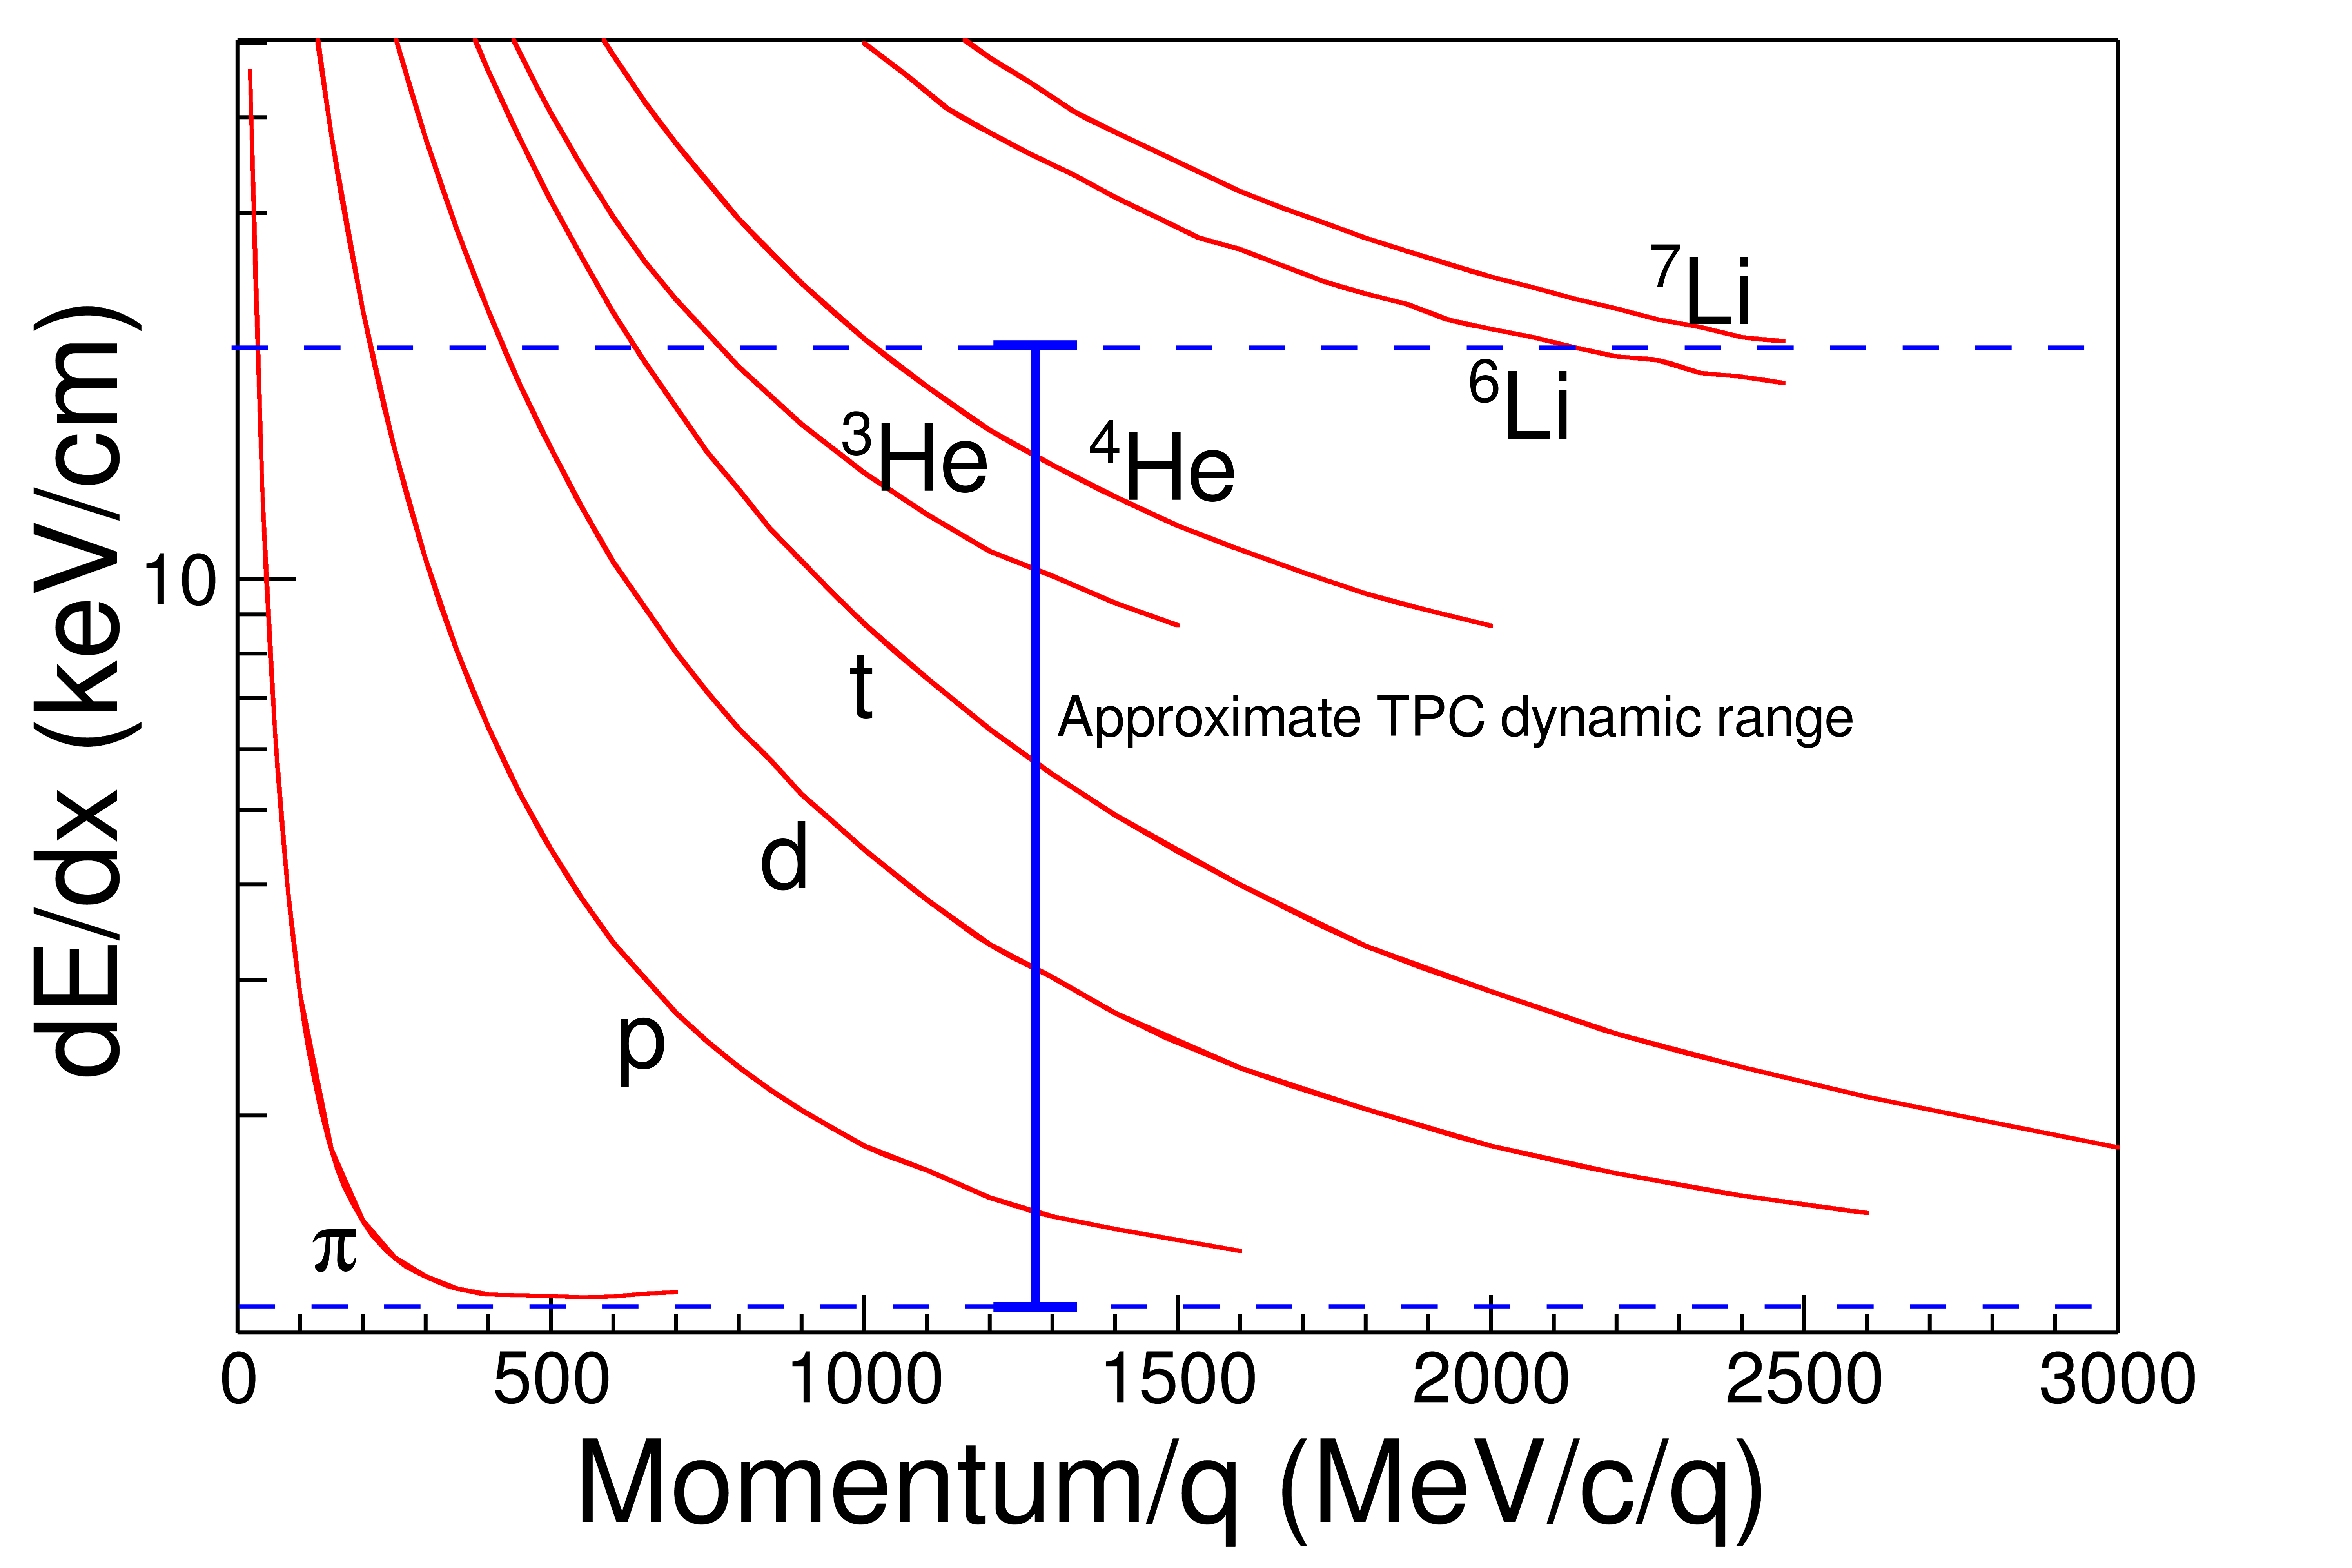
\includegraphics[width=\linewidth]{fig1}
\caption{The expected $dE/dx$ lines of different particles are given in red as calculated by Geant4. The approximate dynamic range of the TPC is shown by the vertical bar for the gain setting used in the experiment. Anything outside of this region would be saturated to some degree.}
\label{fig:intro}
\end{figure}

The rapid increase in the stopping powers at low momentum illustrates the degree to which the effective dynamic range can be exceeded and highlights the problems encountered in studies of intermediate HICs, in which light particles with low momenta are abundantly produced along with highly charged particles. Similar problems are encountered when TPCs are used as active targets in direct reaction studies with rare isotope beams \cite{pattpc}. 

Several techniques have been employed to increase the observable range of energy losses. This can be done by lowering the electronics gain of selected readout channels, or by changing the gas amplification at the readout plane in certain areas of the TPC. In the EOS TPC \cite{eos} this was done by decreasing the voltages in select anode wires in the multi-wire readout. With the prototype Active Target TPC lowering or increasing the gain was achieved by decreasing or increasing the electric fields on selected pads within a Micromegas \cite{pattpc}. The results of changing the gas-gain, or the electronics gain, are rather similar in that reducing the gain to sample a range of higher energy loss makes the TPC effectively blind to minimum ionizing particles in  the regions of lower gain.

While future developments may ultimately provide means to significantly improve the dynamic range of TPC electronics, it is useful to consider whether software strategies can be developed to compensate for the dynamic range limitations of existing devices. In this paper, we illustrate one approach to expand the dynamic range within the context of a standard multi-wire TPC, without the need of extra hardware or dedicated regions of lower gain.


\subsection{TPC Overview}
We begin our discussion by describing some basic properties of the S$\pi$RIT TPC \citep{shane}. It is a rectangular TPC with 12,096 pads designed to constrain the density dependence of the nuclear symmetry energy at densities on the order of twice the saturation density. In order to study central collisions of Sn isotopes at 270 AMeV, the TPC was designed to identify isotopes from Z=1$\sim$3 with the ability to detect minimum ionizing particles such as pions. 

For ease of illustration and discussion in this paper, we use a coordinate systems for the S$\pi$RIT TPC, that has the beam traveling along the +$z$ direction. The positive $y$ axis points away from the drift volume and is also the direction of the magnetic field. The $x$ axis runs parallel to the wires as defined in the right handed coordinate system in Fig.~\ref{fig:padwire}.

\begin{figure}[ht!]
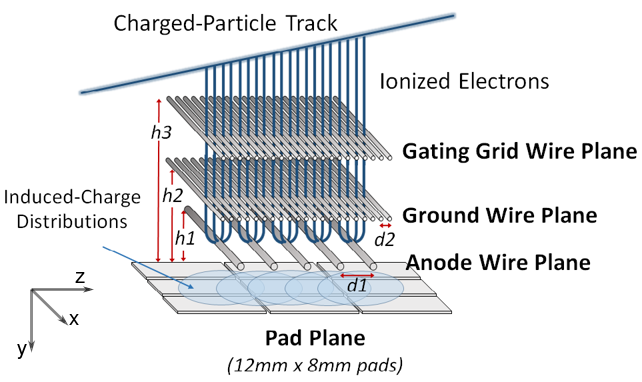
\includegraphics[width=\linewidth]{fig2}
\caption{Cartoon showing the 3 wire planes and a section of the pad plane. The  electron drift lines are shown for the electrons produced from a charge particle passing through the gas volume. $h1$ = 4 mm, $h2$ = 8 mm, $h3$ =14 mm, $d1$ = 4 mm, $d2$ = 1 mm.}
\label{fig:padwire}
\end{figure}

\subsection{Configuration of the pad and wire planes} 
The S$\pi$RIT TPC pad plane is composed of rectangular charge sensitive pads, each with an $x$ dimension of 8 mm, and a $z$ dimension of 12 mm. These pads are arranged in a grid measuring 112 by 108 pads with a total area of 1344~mm~x~864~mm. Each pad is held to the detector ground and serve as an input into the TPC electronics. 

As illustrated in Fig.~\ref{fig:padwire}, there are three wire planes below the pad plane, with the wires aligned along the $x$ axis. The wire plane farthest from the pad plane (14 mm) operates as an ion-gate or a gating grid. Details on the design and operation of the gating grid can be found in \cite{suwat}. The middle wire plane (8~ mm) is grounded. When the gating grid is open, electrons ionized by reaction products in the drift volume move along the $y$ direction along the electric field lines through both the gating grid and ground planes, and eventually avalanche on the anode wires. 

The anode wire plane is closest to the pad plane (4 mm), consisting of 20 $\mu$m diameter wires spaced 4 mm apart. In the vicinity of these wires an avalanche occurs multiplying the secondary electrons on the order of 1000 times, creating electron and ion pairs. In the vicinity of the anode wire the ions move very quickly away due to the high electric fields there. It is this quick motion of the ions in the vicinity of the anode wires that induces image charges on the read-out pads. The distribution of image charges on the pad plane is centered about the avalanche position on the anode wires and its width is fixed by the distance from the anode wire to the pad plane. The ions slow down significantly in the presence of a low electric field (a factor of $10^{-4}$ slower than the electron drift velocity) \citep{blumrol}, which occurs only a couple of $cm$ away from the wire. The induced signal due to this slow motion is filtered out by the pre-amplifier in the electronics. Eventually some of the ions from the avalanche will terminate on the pad plane, while most terminate on the ground and gating grid (most of the time the gating grid is in a closed configuration).



The anode wires are sectioned off into 14 independent sections, each containing 26 wires with 12 sections biased to 1460 V. This setting was optimized to ensure minimum ionizing particles, such as pions, would have a signal to noise ratio of around 20:1. The two remaining sections were biased to 1214 V, reducing the gas gain by a factor of 10, as compared to the other anode sections. As demonstrated by the EOS TPC \citep{eos}, lowering the anode wires effectively extended the dynamic range.  This gain reduction allowed for a direct validation of the new method for extending the dynamic range presented here. 

\subsection{Generic Electronics for TPCs}
The induced charge from each pad are input into one of the 12k charge sensitive pre-amplifiers, it is then shaped and digitized, all by the Generic Electronics for TPCs (GET) system \cite{get}. As details of our implementation of the GET system are described in \citep{aki}, our description of the electronics can be limited to the options relevant to this paper.

The electronics for each pad has a shaping constant of 117 ns and reads out the induced signal on the pads at a 25 MHz sampling rate. The dynamic range of the GET electronics was set to 120 fC and digitized over a 12 Bit ADC range which corresponds to 4096 channels of resolution. The typical rms noise level was about 5 ADC channels about 400 electrons, corresponding to a maximum signal to noise ratio of about 

. 

In the data discussed here, the variations between electronics channels were calibrated by measuring the response of each channel to an injected reference pulse, covering the full dynamic range of each channel, reducing the variations to less than a few percent.
 
\subsection{Analysis Software}
A software package called S$\pi$RITROOT was developed to reconstruct the events in the TPC based on the FAIRROOT container package written in C\texttt{++} \cite{fairroot}. Due to the large number of particles emitted in HICs, there may be several signals coming from tracks passing under the same pad separated only by their arrival time. Using an expected pulse shape, S$\pi$RITROOT fits all the signals within a pad, giving the arrival time and height of the signal for each particular track. The height of the fitted pulse is proportional to the total charge of that event, $Q$, and the $y$-coordinate is calculated as $y = v\cdot t_0$, where $v$ is the drift velocity and $t_0$ the arrival time. We define the $x$ and $z$ position from the center of each pad, and combine the summary of information ($x$,$y$,$z$,$Q$) into a ``hit''. 

 An algorithm then finds the collection of hits belonging to each unique helix track. We then reduce these several adjacent hits along a particluar track into ``clusters''. A cluster's position is defined as the charge-weighted average position of the hits within a cluster, with the total charge of the cluster being the sum of the charges of each hit. The clusters represent our best measurement of the track's path and are then fitted in the GENFIT track fitting package \cite{genfit}, giving the final momentum of the track. A final vertex of the event is fitted from all tracks using the package RAVE \cite{rave}. 
 

\subsection{Definition of clustering}
A brief description of the method of clustering is illustrated in Fig.~\ref{fig:topview}. When the projection of a track onto the pad plane is passing nearly parallel to the $z$ axis, little can be learned from the distribution of hits along the $z$ axis; precise position information can be obtained from the mean value of the hit distribution along the $x$ axis. If the segment of a track is traveling along the $x$ axis, little can be learned from the $x$ distribution while the precise position can be estimated from the hits along the $z$ axis. We have illustrated this as the three clusters at the bottom of Fig.~\ref{fig:topview} are clustered along the $x$ axis and the upper three are along the $z$ axis, as shown by the bolded pads for one of the clusters in each direction.


\begin{figure}[ht!]
\centering
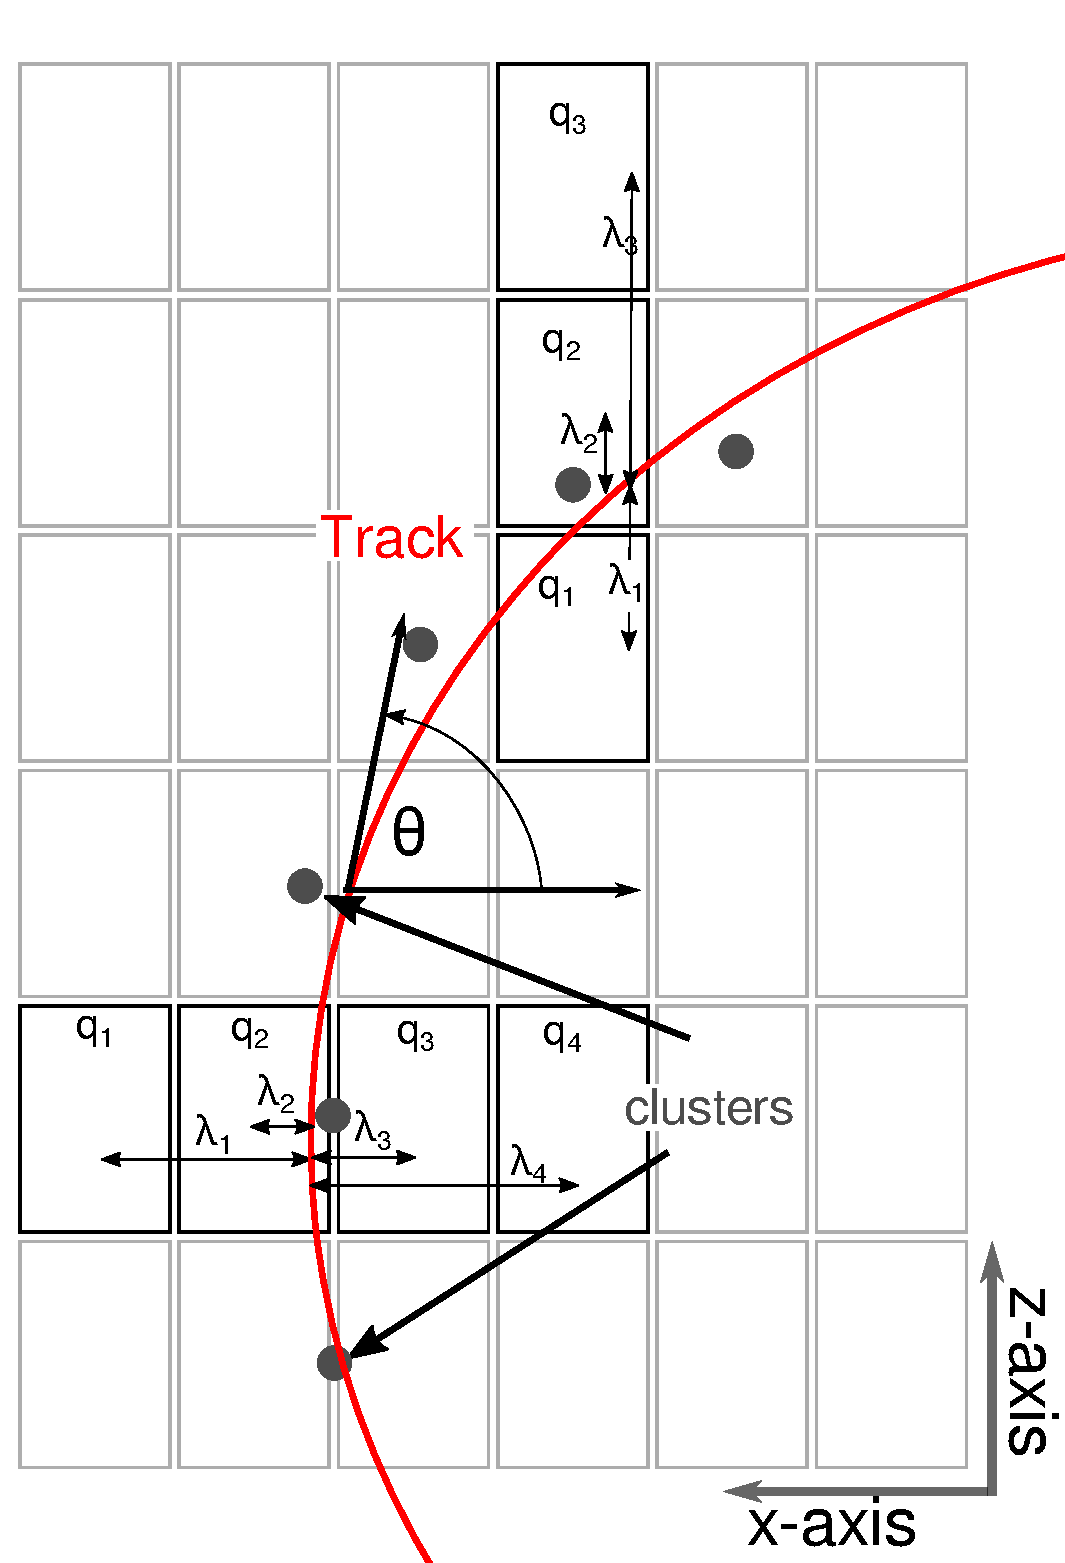
\includegraphics[scale=.35]{fig3.pdf}
\caption{Cartoon of a top down view of a fit to a track passing through several pads. The bolded pads and the charges $q_i$ represent the hits belonging to that pad and the clusters of the track representing the average position of the track. The three clusters at the bottom are clustered in the $x$-direction for the upper three are clustered in the $z$-direction. The estimated position of the avalanche is given by the track fit, and the position from the center to each pad to the $\bar{x}$ position is given as $\lambda_i$.}
\label{fig:topview}
\end{figure}

We define the clustering direction depending on the angle of the track, at the point of each cluster, with respects to the $x$ axis, defined as $\theta$. For example, the crossing angle is defined as $90^{\circ}$ for a track going along the $z$ axis, and $0^{\circ}$ for a track going along the $x$ axis. In the case that the crossing angle is $45^{\circ} < \theta \leq 90^{\circ} $ the clustering direction is along the $x$ axis. For $0^{\circ} < \theta \leq 45^{\circ}$ it is along the $z$ axis. 

 The position along the clustering direction is calculated by weighting the individual hit's positions by their charges $q_i$ and getting the mean value. The other direction is set to the center of the pad. For example, if we are clustering along the $x$ axis for a cluster, the $z$-position is set to the center of the pad in the $z$-direction and vice versa. 
 


\begin{figure}[ht!]
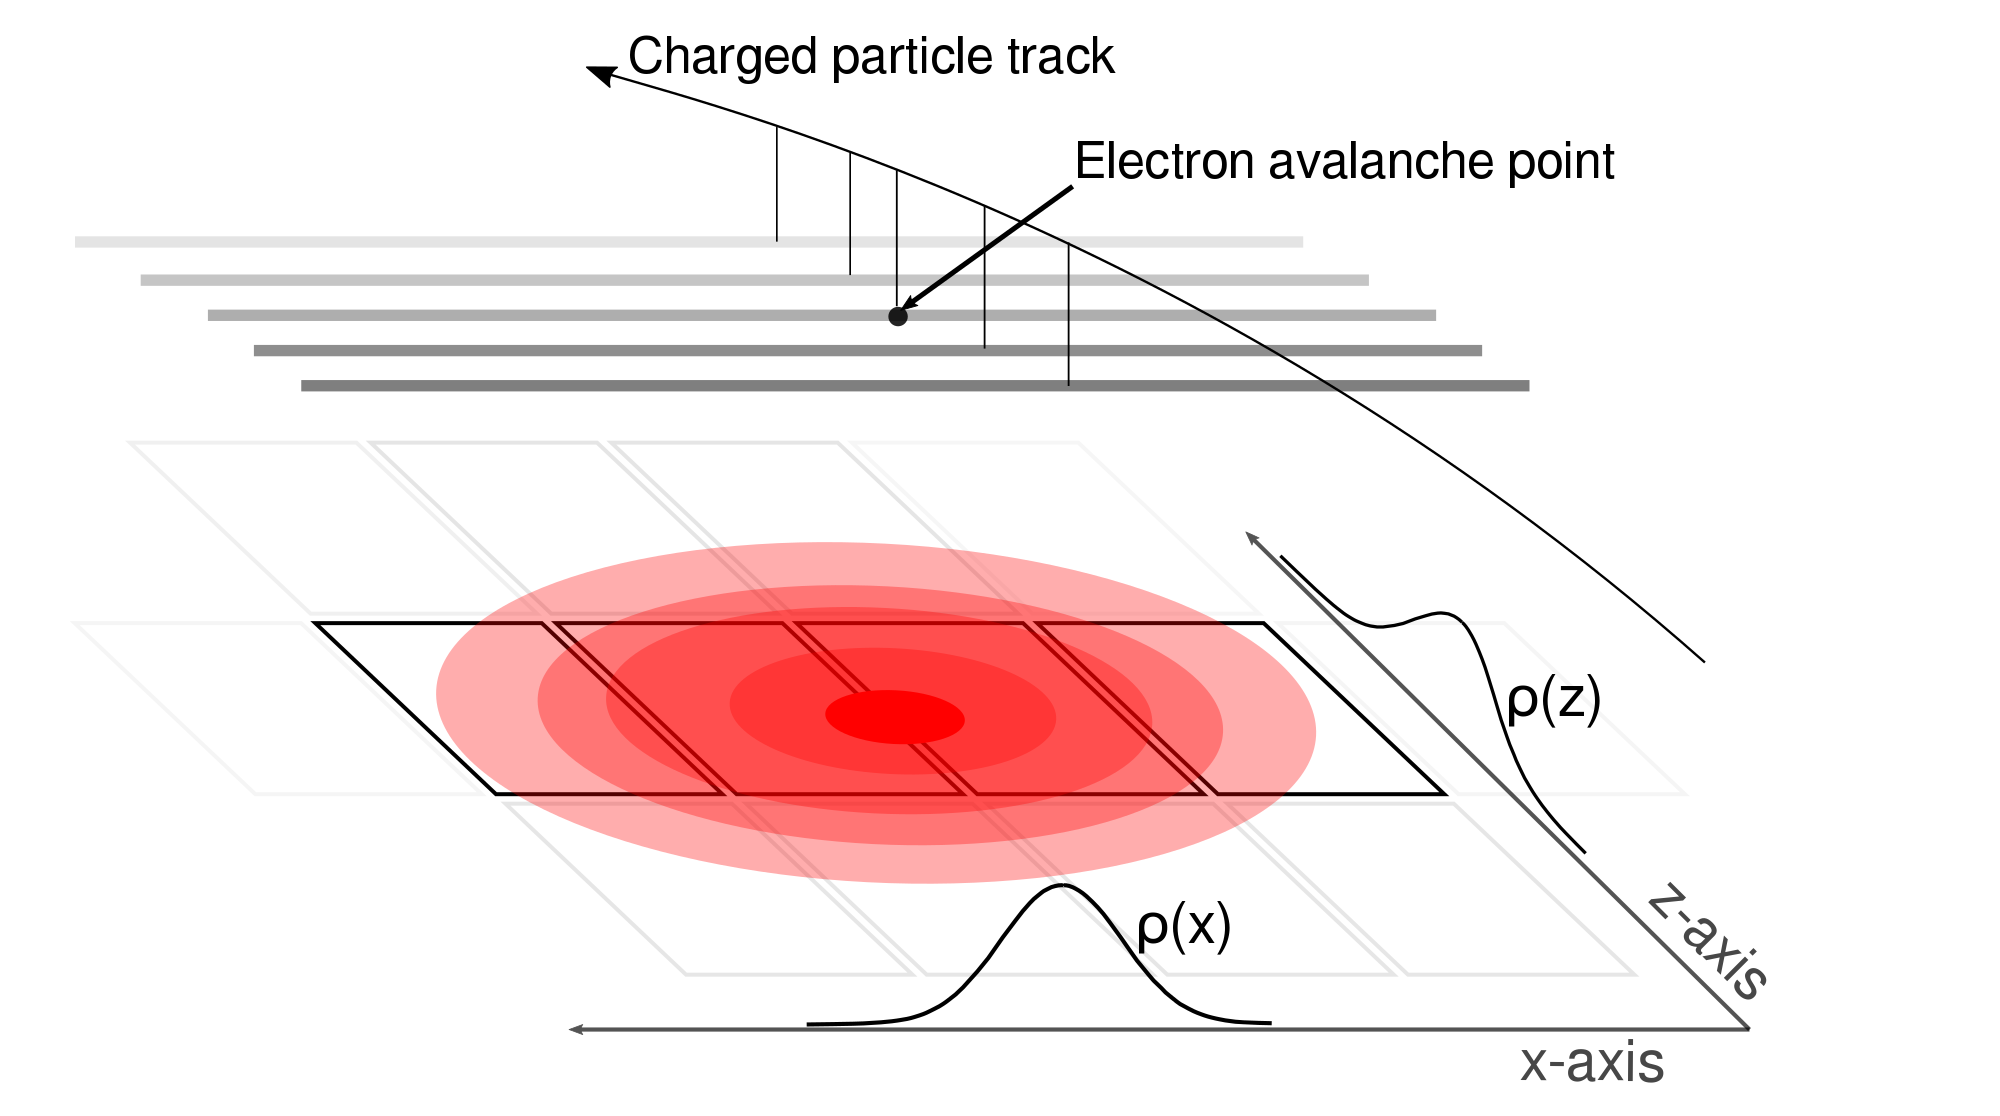
\includegraphics[width=\linewidth]{fig4}
\caption{A cartoon illustration of the charge distribution resulting from an electron avalanche on one wire and the projections of the distribution onto the two axis $\rho(x)$ onto the $x$ axis and $\rho(z)$ onto the $z$ axis. The orientation of the wire planes is flipped upside down to display the perspective better.}
\label{fig:prf}
\end{figure}

\section{Pad Response Function}
The charge distribution on the pad plane resulting from an electron avalanche is two dimensional, as illustrated in Fig.~\ref{fig:prf}, with the projections onto the $x$ and $z$ axis of this distribution labeled as $\rho(x)$ and $\rho(z)$ respectively. The charge observed on each pad is the integral of this distribution over the pad's dimensions, which is called the Pad Response Function (PRF).

In this example the clustering direction would be along the $x$ axis, as illustrated by the bolded pads. By choosing to cluster only in one direction, we have not included the charge in adjacent pads along the $z$ axis resulting from the tails of $\rho(z)$. Therefore the charge not included in the the bolded pads will be incorporated into adjacent clusters, introducing small correlations in charge between neighboring clusters. 


\subsection{Gatti Pad Response Function}
Gatti \cite{gatti} derived a semi-empirical formula for the charge distribution in a simple multi-wire TPC. The function given in Eq.~\ref{eq:gatti}, depends only on the width of a pad ($w$), the distance of the anode plane to the pad plane ($h$), and the distance of the pad center to the avalanche point $\lambda$. It is a single parameter equation where the two parameters $K_1 = \frac{K_{2}\sqrt{K_3}}{4 \arctan(\sqrt{K_3})}$ and $K_2 = \frac{\pi}{2}\left(1-\frac{\sqrt{K_{3}}}{2}\right)$ depend on the parameter $K_3$, which is a function of the ratio of the anode wire diameter to the distance of the anode wires to the pad plane. $K_3$ can be looked up in a graph in \cite{blumrol} and \citep{gatti}.

\begin{equation}\label{eq:gatti}
\begin{split}
PRF_{\mathrm{Gatti}}(\lambda)
& = \frac{K_{1}}{K_{2}\sqrt{K_{3}}}\bigl[\arctan(\sqrt{K_{3}}\tanh\bigl[K_{2}\bigl(\frac{\lambda}{h}+\frac{w}{2h}\bigr)\bigr]) \\
& - \arctan(\sqrt{K_{3}}\tanh\bigl[K_{2}\bigl(\frac{\lambda}{h}-\frac{w}{2h}\bigr)\bigr])\bigr] \\
\end{split}
\end{equation}

\subsection{Experimental Pad Response Function}

The correlations we introduced by only clustering along one direction do not play a significant role in the particle identification, but cause deviations from the expected Gatti distribution. Also, analytic PRFs only exist for classical multi-wire TPCs. For these reasons it is useful to experimentally measure the PRF and fit it with an empirical function, typically a Gaussian, to describe its behavior. 

As in Fig.~\ref{fig:topview}, we postulate that the PRF is a function of the total charge deposited in a cluster $Q = \sum_i q_i$, and the difference in position of the center of the $i^{th}$ pad, $x_i$, to the mean position $\bar{x} = \sum_i x_i q_i/Q$, defined as $\lambda_i = x_i-\bar{x}$. The PRF is simply defined as the charge fraction of each pad as a function of $\lambda$, as shown in Equation \ref{eq:prf}. 

\begin{equation}\label{eq:prf}
PRF(\lambda_i) = \frac{q_i(\lambda_i)}{Q}
\end{equation}

Averaging over many events in the experimental data, the resulting PRF for the S$\pi$RIT TPC is shown in Fig.~\ref{fig:expprf}. Here we see the deviations from the expected analytic Gatti distribution (black curve), whereas fitting with a two parameter Gaussian function (red curve) gives a better description of the  data, Eq.~\ref{eq:gaus}, with the two parameters being the normalization coefficient, $N_0$, width $\sigma$, and with a mean value assumed to be 0.

\begin{equation}\label{eq:gaus}
PRF_{\mathrm{Gaus}}(\lambda) = N_0 e^\frac{-\lambda^2}{2\sigma^2}
\end{equation}

\begin{figure}[ht!]
\begin{overpic}[width=\linewidth]{fig5.pdf}
\put(61,55){\contour{white}{ PRF${}_{\mathrm{Gaus}}(\lambda)$ eq. \ref{eq:gaus}  }}
\put(61,49){\contour{white}{ PRF${}_{\mathrm{Gatti}}(\lambda)$ eq. \ref{eq:gatti} }}
\end{overpic}
\caption{Experimental pad response function of many events for a crossing angle of $85^{\circ} < \theta \leq 90^{\circ}$.  }
\label{fig:expprf}
\end{figure}

\section{Pad Response Function vs. crossing angle}
The shape of the PRF depends on the crossing angle of the track \citep{gatti}. Plotted in Fig.~\ref{fig:prfangle} is the PRF of $\pi^-$ tracks vs. the crossing angle $\theta$. The PRF gets wider starting from $90^{\circ}$  and going to $45^{\circ}$; if we did not switch clustering directions the PRF would become wider until it was a uniform distribution and there was no position resolution. Since we switch the clustering direction from $x$ to the $z$ direction at $45^{\circ}$, the opposite trend is seen where the PRF becomes narrower as the position resolution gets better going from $45^{\circ}$ to $0^{\circ}$.

\begin{figure}[ht!]
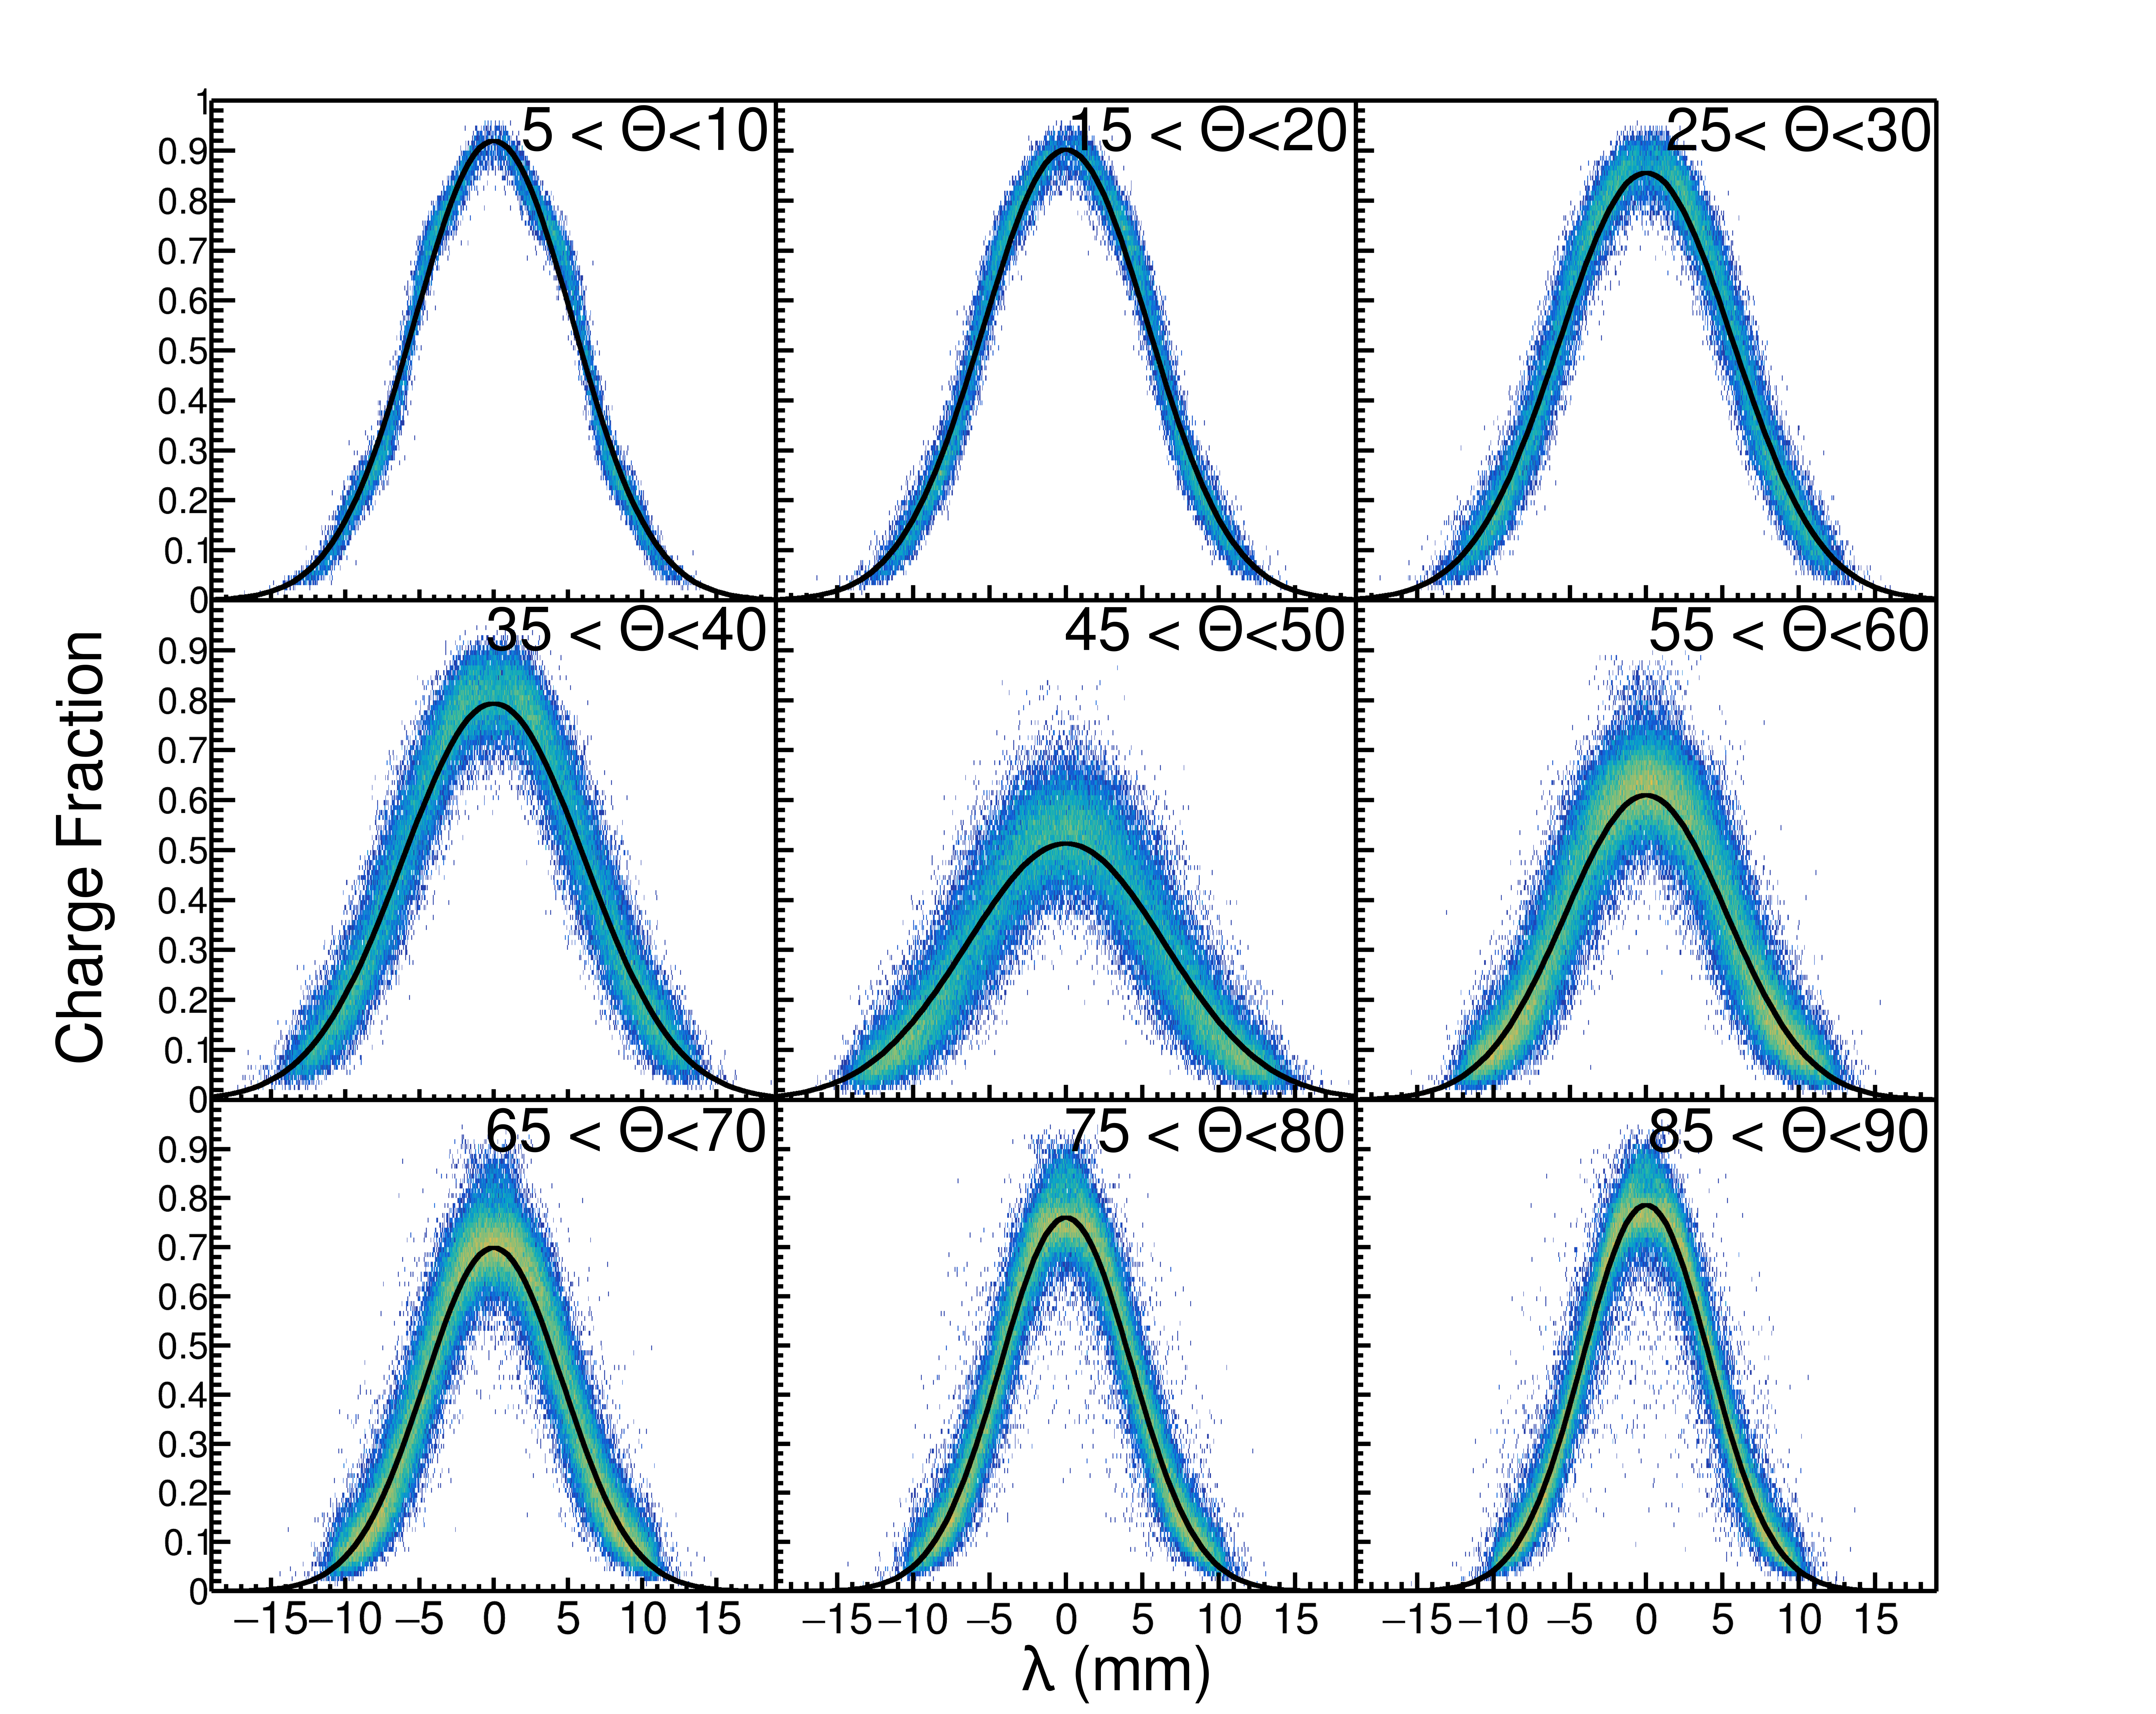
\includegraphics[width=\linewidth]{fig6}
\caption{Experimental pad response function as a function of the crossing angle $\theta$ with the corresponding fits.}
\label{fig:prfangle}
\end{figure}


\begin{figure}[ht!]
\vspace{5mm}
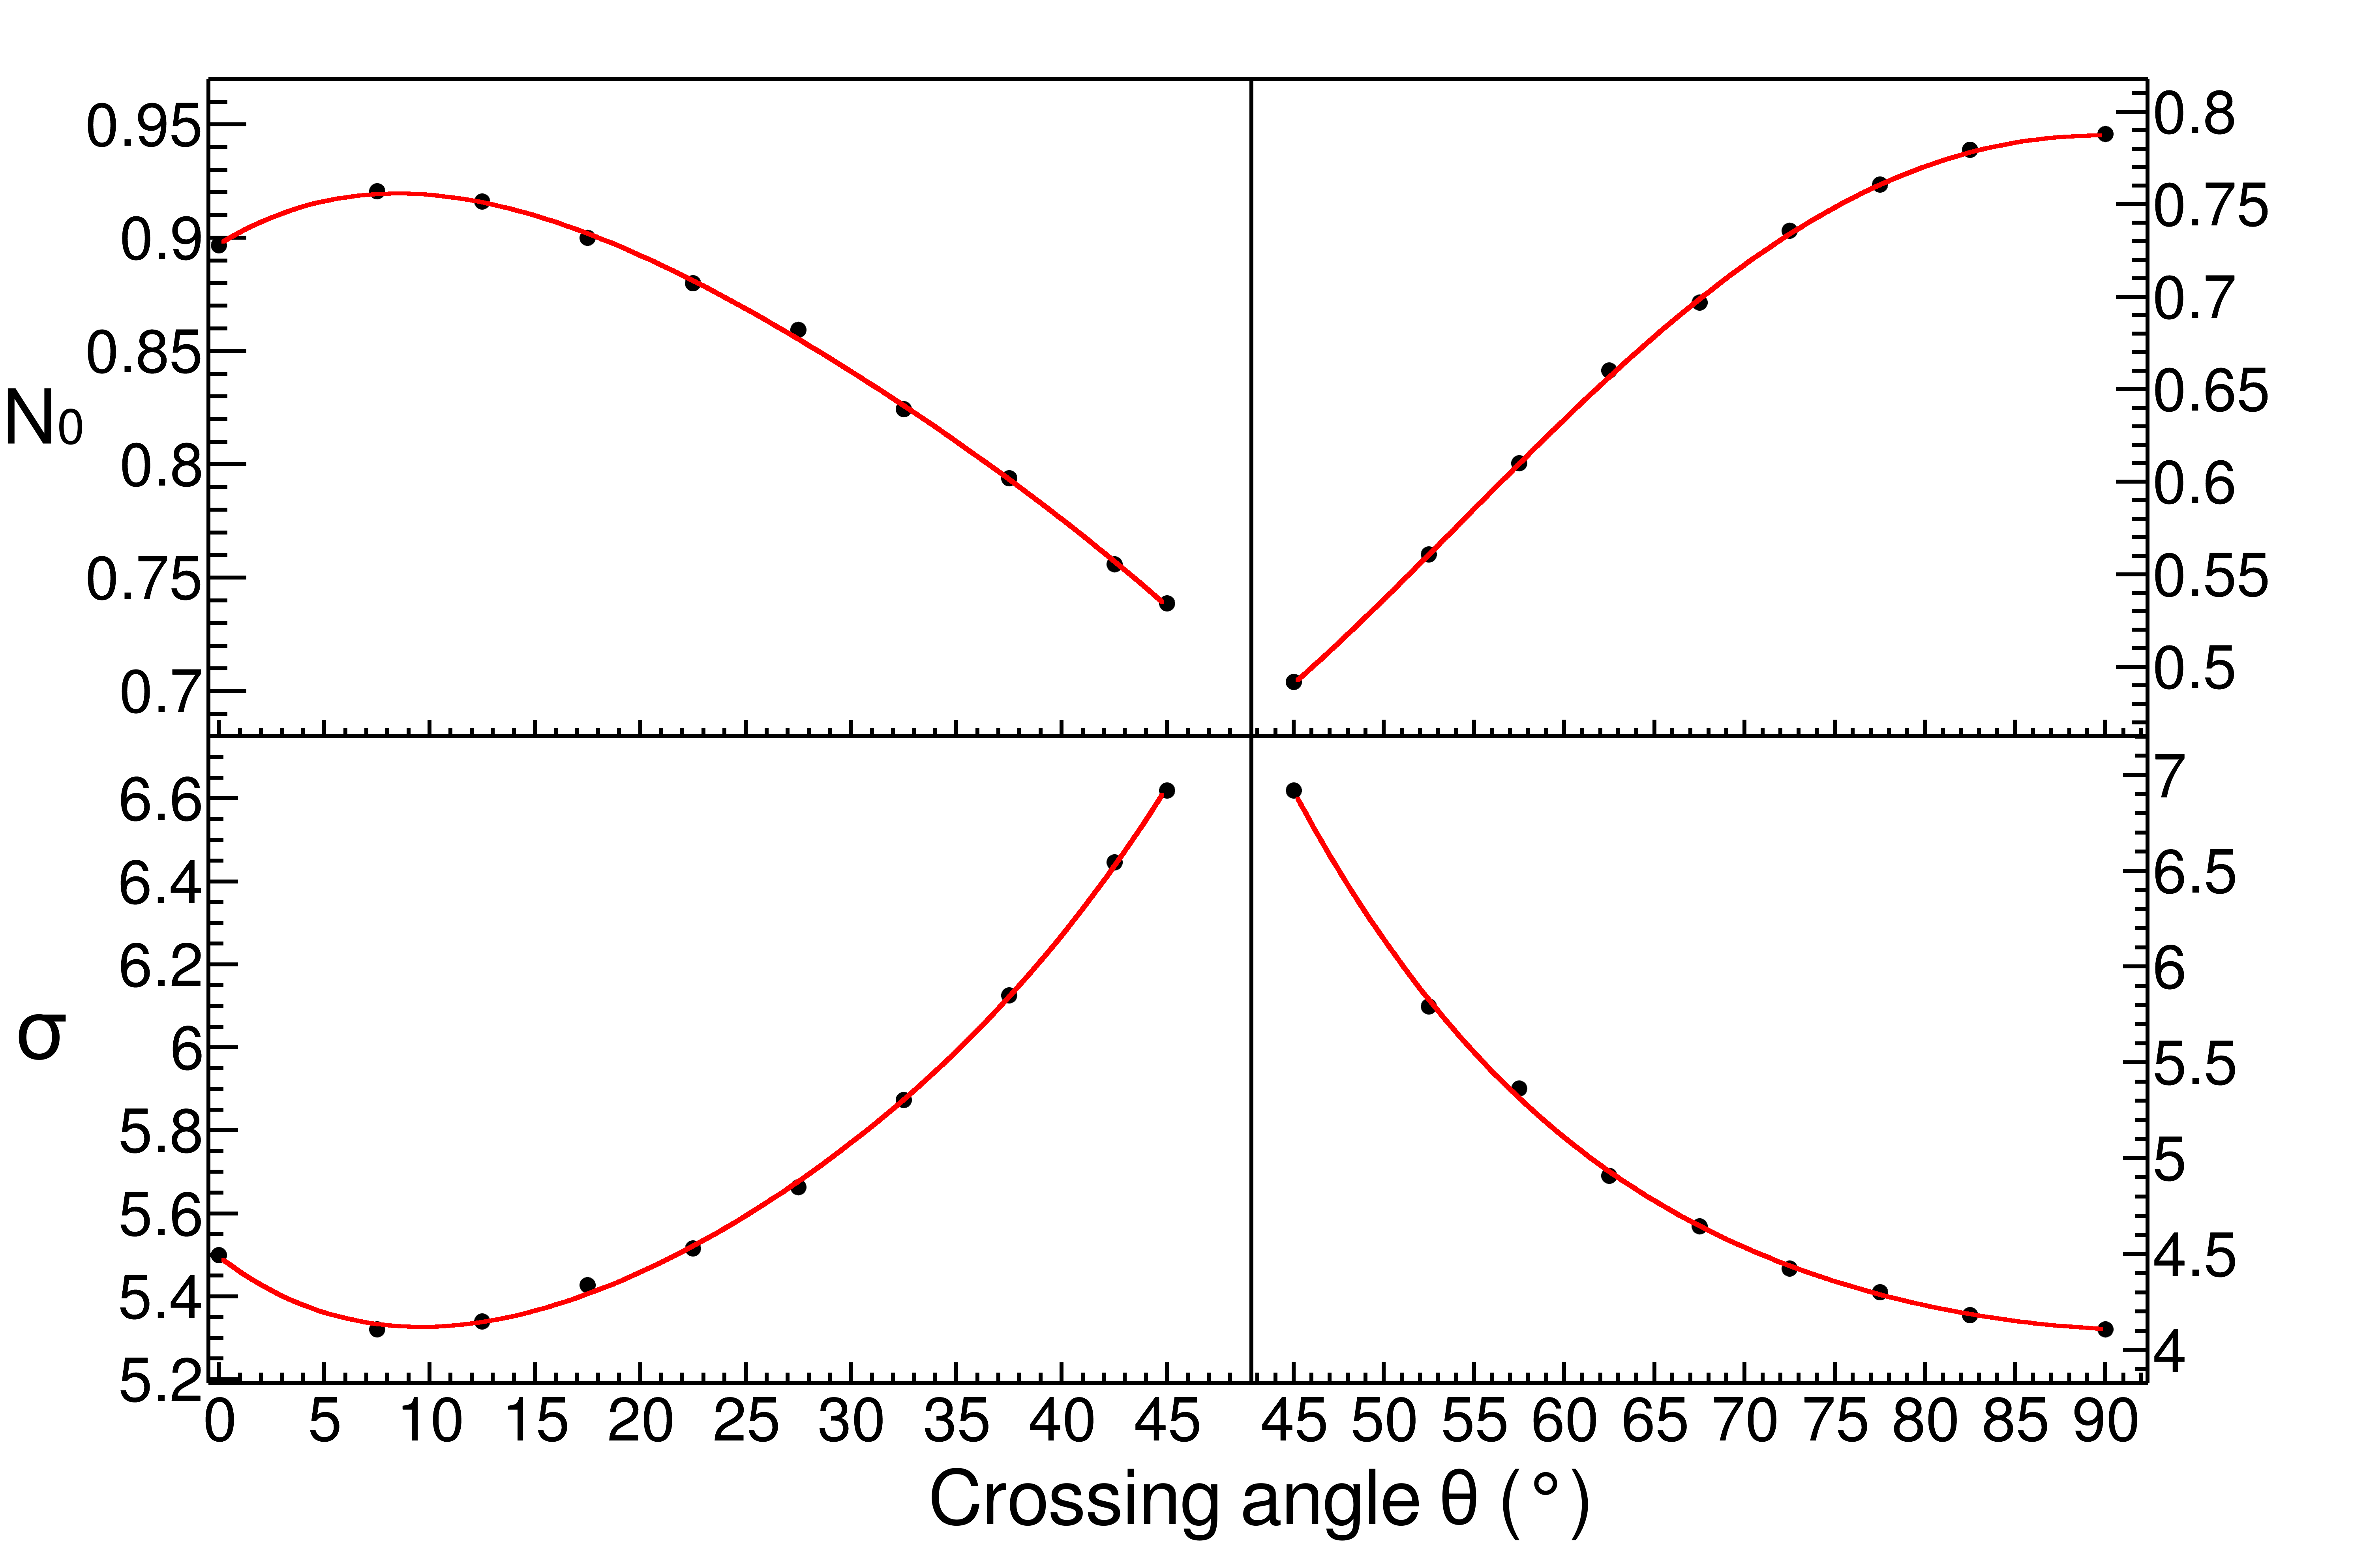
\includegraphics[width=\linewidth]{fig7}
\caption{Parameters $N_{0}$ and $\sigma$ as a function of the crossing angle $\theta$ with the $4^{th}$ order polynomial fits.}
\label{fig:normsigma}
\end{figure}

\begin{comment}
\begin{table}
\centering
 \begin{tabular}{||c c c c c c||} 
 \hline
 Coefficient & $c_0$ & $c_1$ & $c_2$ & $c_3$ & $c_4$ \\ [0.5ex] 
 \hline\hline
 $0 < \theta < 45$ & & & & &  \\ [.25ex]
 \hline
 $N_0$ & .897 & 5.766E-3 & -4.263E-4 & 7.444E-6 & 5.705E-8 \\ 
 \hline
 $\sigma$ & 5.496 & -3.920E-2 & 2.693E-3 & -5.208E-5 & 5.334E-7\\
 \hline
 $45 < \theta < 90$ & & & &  & \\ [.25ex]
 \hline	
 $N_0$ & 1.220 & -6.258E-2 & 1.608E-3 & -1.492E-5  & 4.654E-8 \\
 \hline
 $\sigma$ & 31.368 & -1.109 & 1.779E-2 & -1.336E-4 & 3.940E-7\\
 \hline
\end{tabular}
\caption{Coefficients of the $4_th$ order polynomial fit to the Gaussian parameters $N_0$ and $\sigma$. The polynomial form is given as $c_0 + c_1 x + c_2 x^2 + c_3 x^3 + c_4 x^4$}
\label{tb:coeff}
\end{table}
\end{comment}
 
Fits were performed to the experimental data with  $5^{\circ}$ width bins from $0^{\circ} < \theta \leq 90^{\circ}$. The two parameters of the Gaussian fits are plotted versus $\theta$ in Fig.~\ref{fig:normsigma}; a $4^{th}$ order polynomial fit between these points allowed for interpolating between $\theta$.

\section{Method of Desaturation}
We will use the term ``desaturation'' for our process of correcting the charge values of the saturated pads. Figure \ref{fig:satpad} shows a typical situation of saturated signals. When an avalanche causes a large induced signal, the pads directly underneath collect the largest charge becoming saturated, denoted as $q_{2'}$ and $q_{3'}$. Pads further away experience smaller, non saturating charges, denoted as $q_{1}$ and $q_{4}$. Though we do not know the saturated charge values, the distribution of all charges must follow the PRF which we have experimentally measured. From the clusters crossing angle, we can get the corresponding parameters for the PRF as described above and in Fig.~\ref{fig:normsigma}.

We assume the distance of each pad to the track, $\lambda_i$, is fixed, defining the fraction of charge each pad receives as given by the $PRF(\lambda_i)$ function. 


\begin{equation}\label{eq:chi}
\chi^2 = \sum_i \frac{(q_i^{\mathrm{obs}} - q_i^{\mathrm{expect}})^2}{q_i^{\mathrm{expect}}}
\end{equation}


To determine the best estimate for the charge values of each saturated pad, a chi squared function is minimized, given in  Equation \ref{eq:chi}, where $q_i^{\mathrm{obs}}$ are the observed, non-saturated charges $q_{1}$ and $q_{4}$, and $q_i^{\mathrm{expect}}$ are the charges we expect to observe, calculated as $q_i^{\mathrm{expected}} = Q\cdot PRF(\lambda_i)$. The charges $q_{2'}$ and $q_{3'}$, make up the unknown variable and are allowed to vary in the $\chi^2$ minimization, where they are added to make up the total expected charge $Q$.


\begin{figure}[ht!]
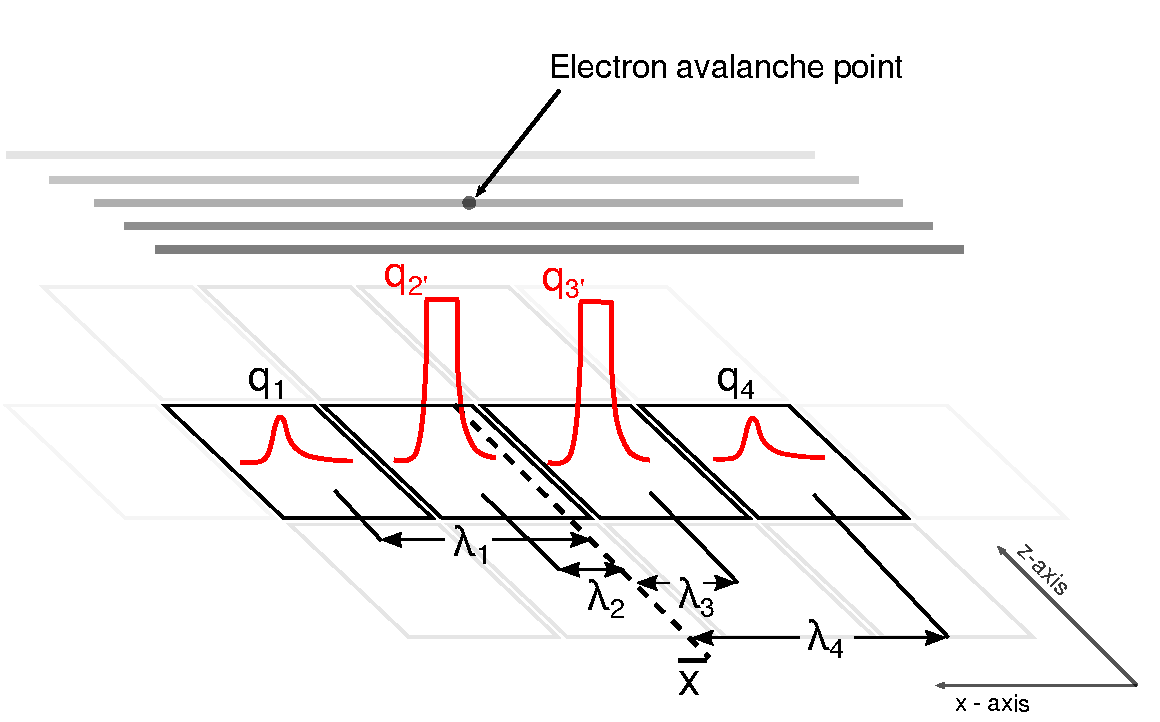
\includegraphics[width=\linewidth]{fig8.pdf}
\caption{A typical case of a saturating event. The red pulses represent the time bucket signal for each collected charge. The pads directly underneath the avalanche point, $q_{2'}$ and $q_{3'}$, are saturated while pads farther away, $q_1$ and $q_4$ are not saturated.}
\label{fig:satpad}
\end{figure}

\section{Experimental data}
Two sets of data were used for the testing and validation of this method. A cocktail beam consisting of (p, d, t, ${}^3$He, ${}^4$He, ${}^6$Li, ${}^7$Li) light charged particles was injected into the TPC for calibration purposes, and tuned to two different rigidity, $B\rho$ settings. The momentum resolution was approximately 1\%, as determined by the slits of the BigRIPS fragment separator of the Radioactive Isotope Beam Factory (RIBF) in RIKEN \cite{bigrips}. A 21 mm thick aluminum target was inserted for part of the lower $B\rho$ setting, further degrading the energy of the beam for a third calibration point. 

Shown in Fig.~\ref{fig:cocktail} is a typical cocktail event, where one particle enters the TPC volume at a time and parallel to the pad plane, representing an ideal case for momentum and $dE/dx$ determination; as it does not suffer from inefficiencies of high multiplicity events seen in the collision experimental data.  

\begin{figure}[ht!]
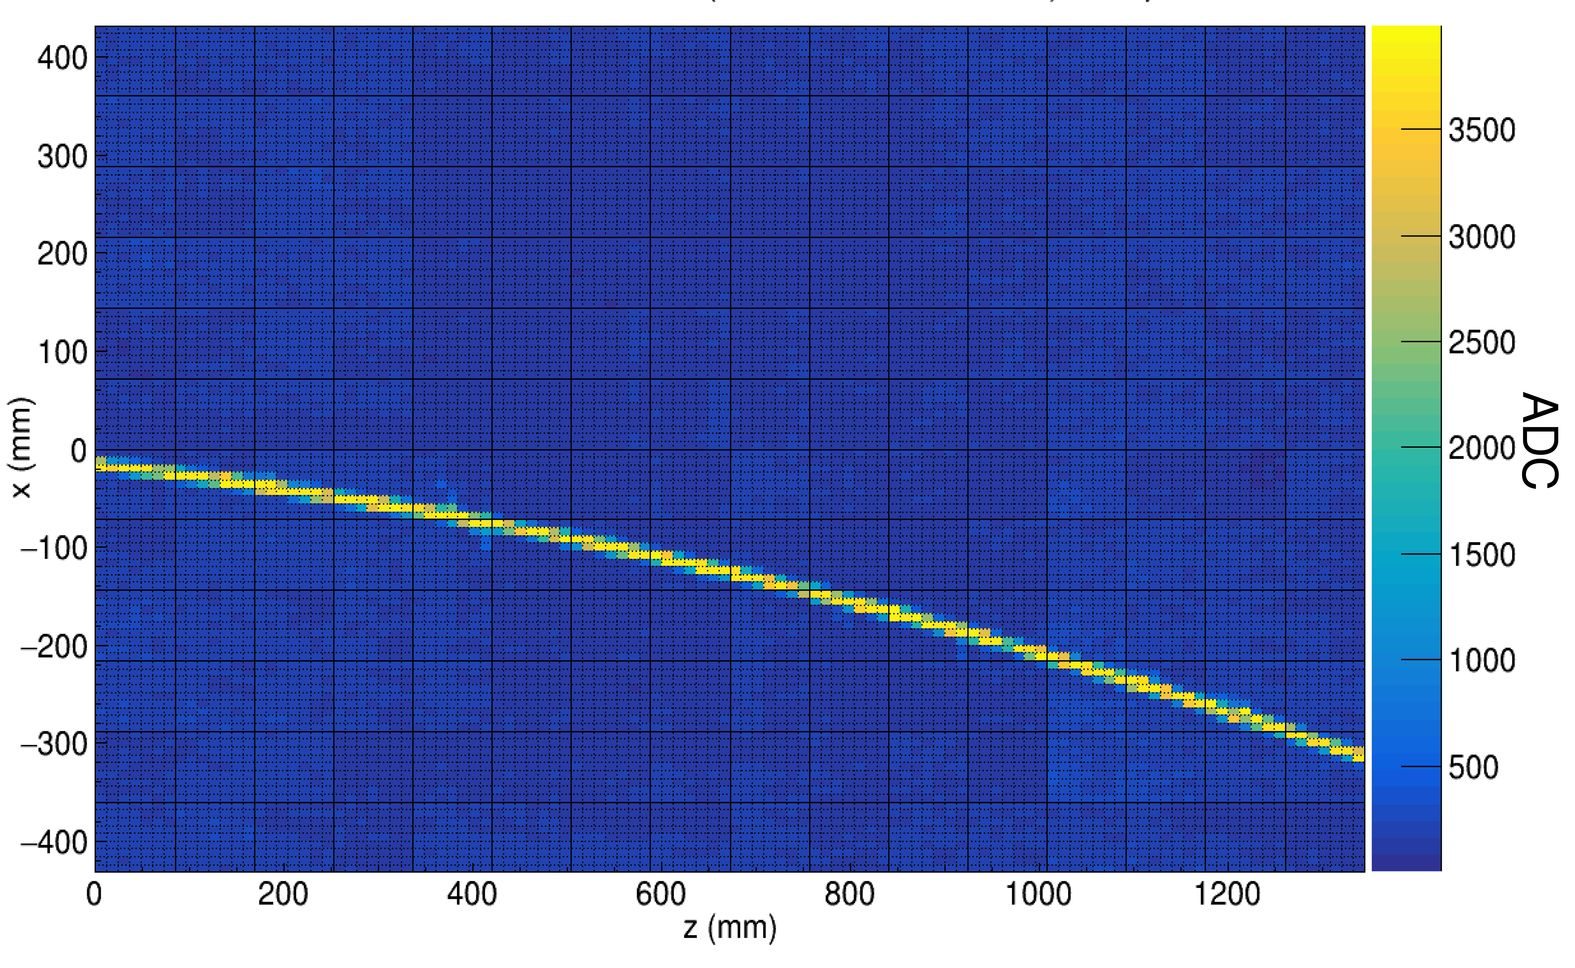
\includegraphics[width=\linewidth]{fig9}
\caption{Pad plane projection for a cocktail event in the TPC.}
\label{fig:cocktail}
\end{figure}

\begin{figure}[ht!]
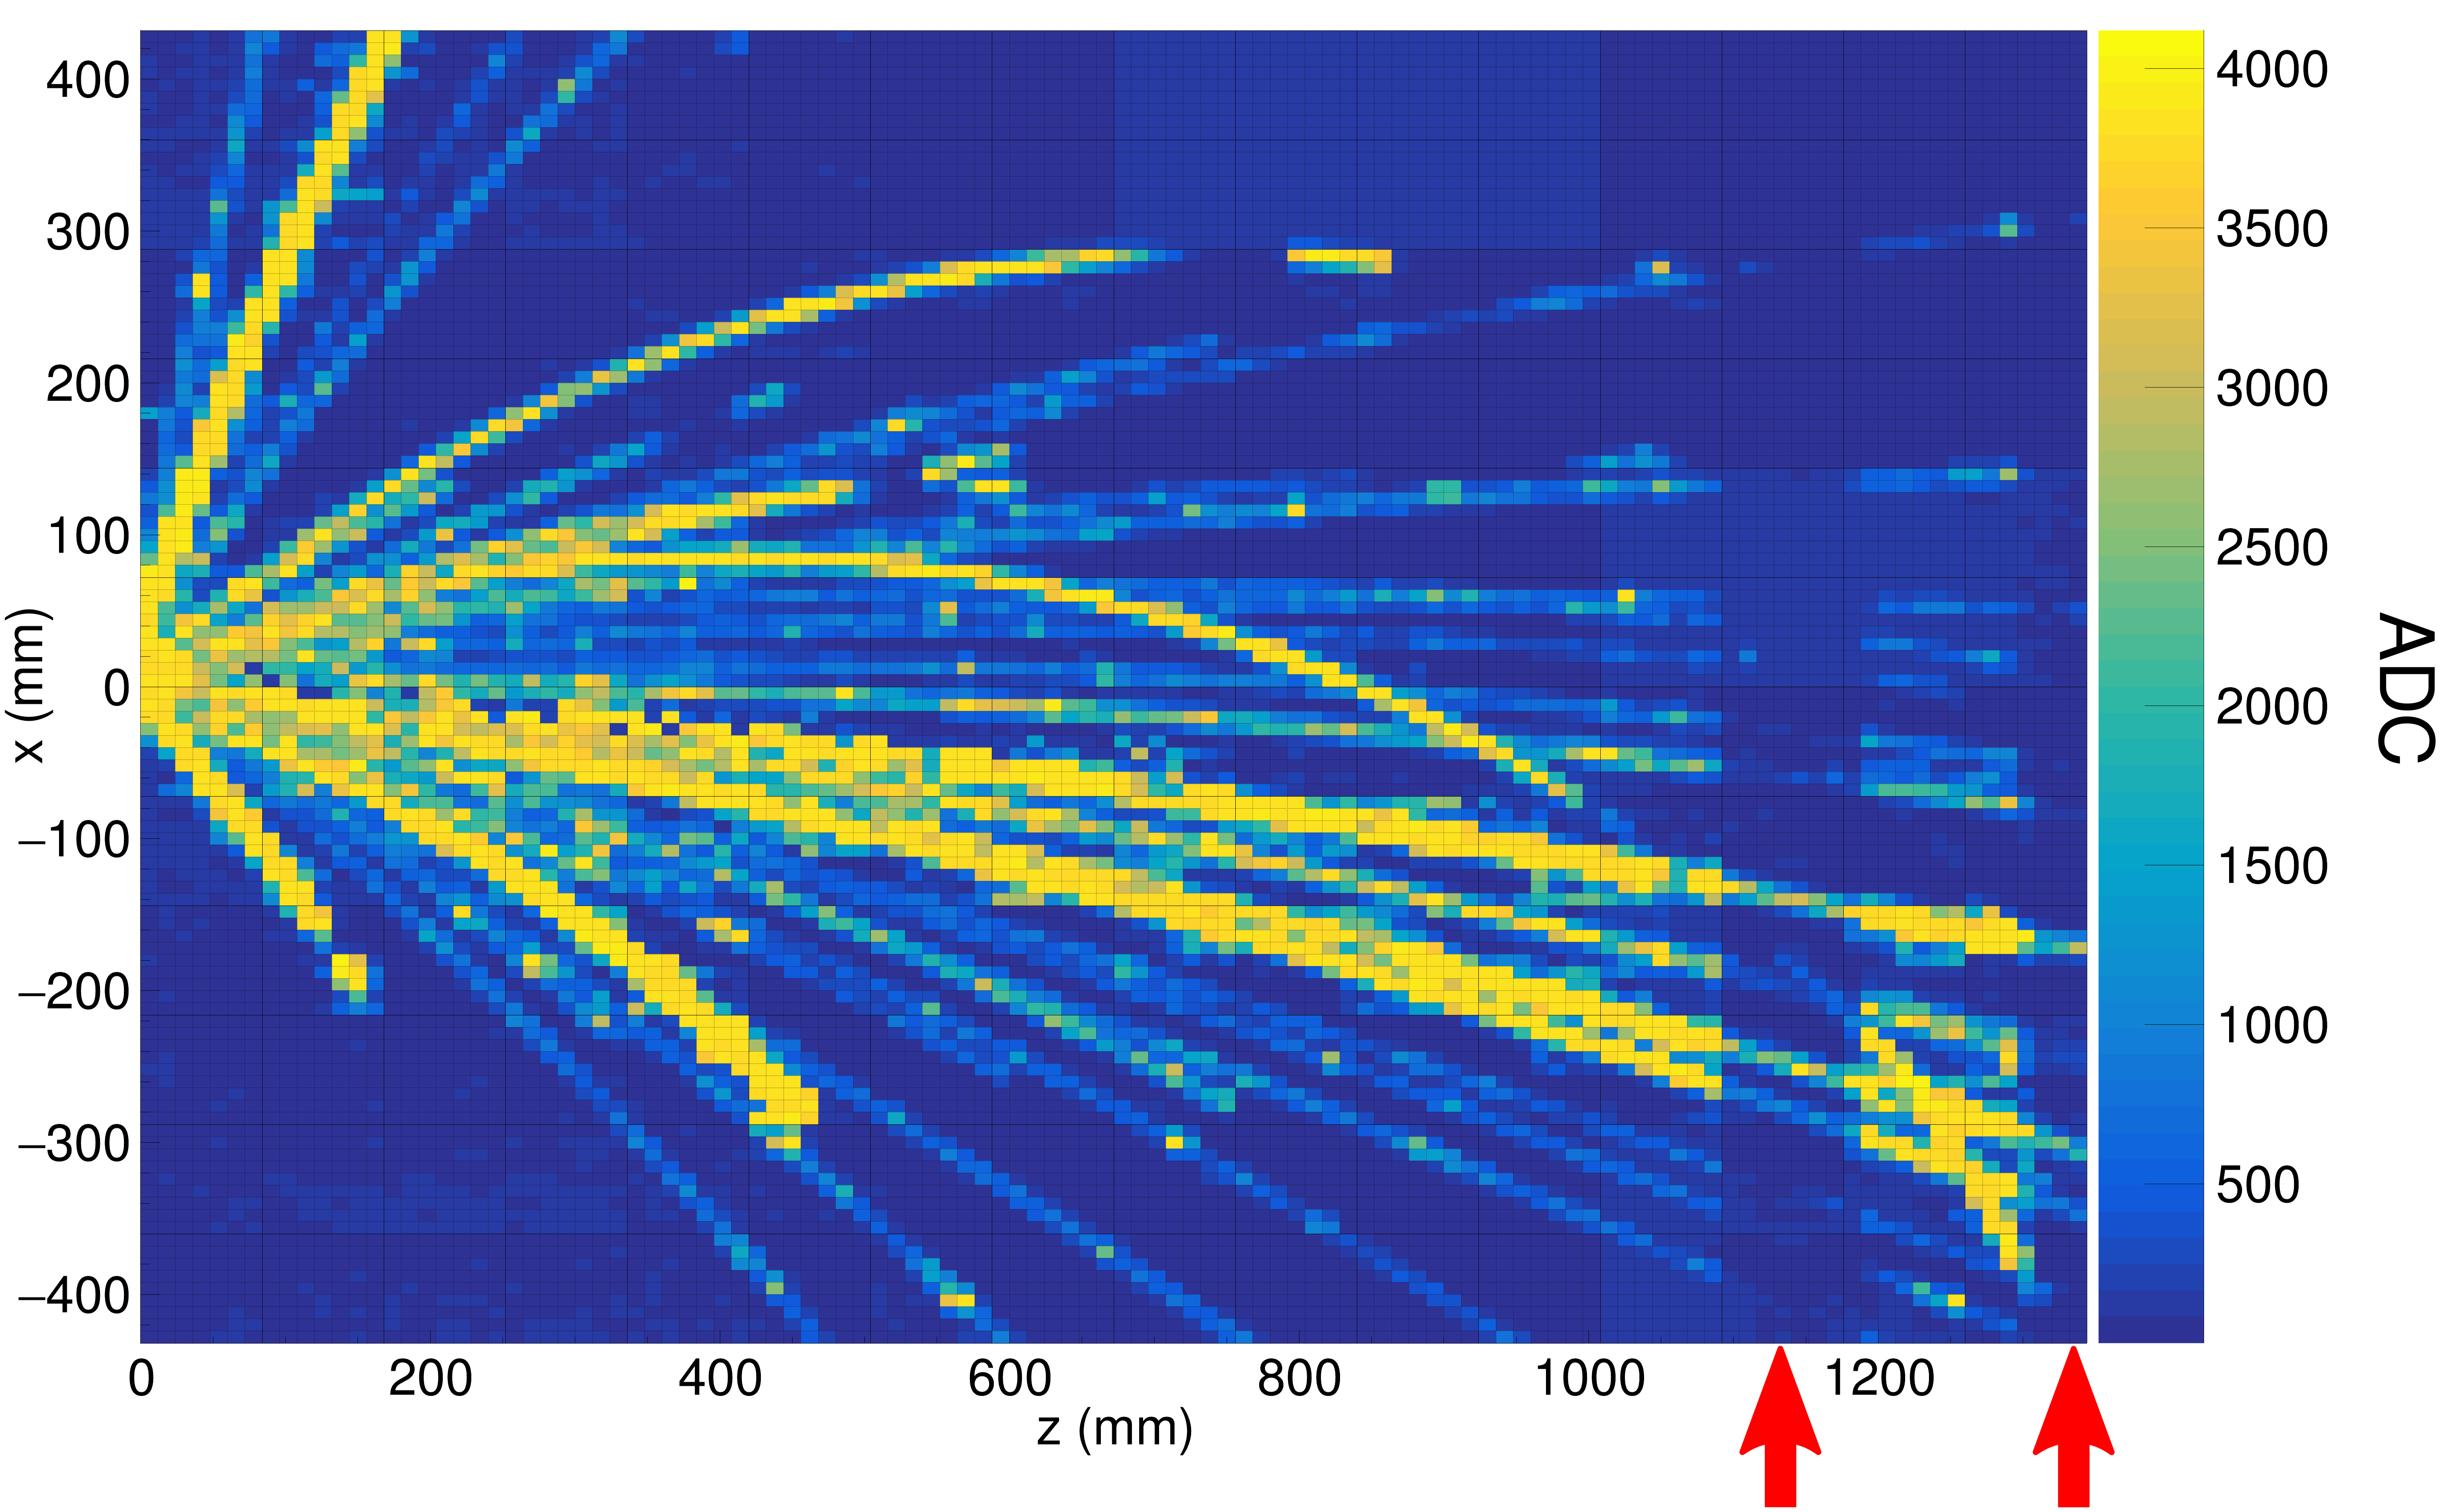
\includegraphics[width=\linewidth]{fig10}
\caption{Pad plane projection for a collision event in the TPC. Highlighted by red arrows are two regions of anode wires which had a reduced voltage of 1214 V. The voltage of the rest of the TPC anode wires are 1460 V. The reduction in voltage reduces the gain by a factor of about 10. }
\label{fig:data}
\end{figure}



The other type of data was the collision of a ${}^{132}$Sn beam onto a ${}^{124}$Sn target triggered on central nuclear collisions. Shown in Fig.~\ref{fig:data} is the typical pad plane response for a central nuclear collision. During the experiment the voltages of two anode sections (as indicated by red arrows in Fig.~\ref{fig:data}) were biased to 1214 V. The gain of these sections were also reduced by a factor of about 10 times as compared with the other sections which were biased to 1460 V. We refer to the 1460 V region as high gain and the 1214 V region as low gain. 

\begin{figure*}[t]
\centering
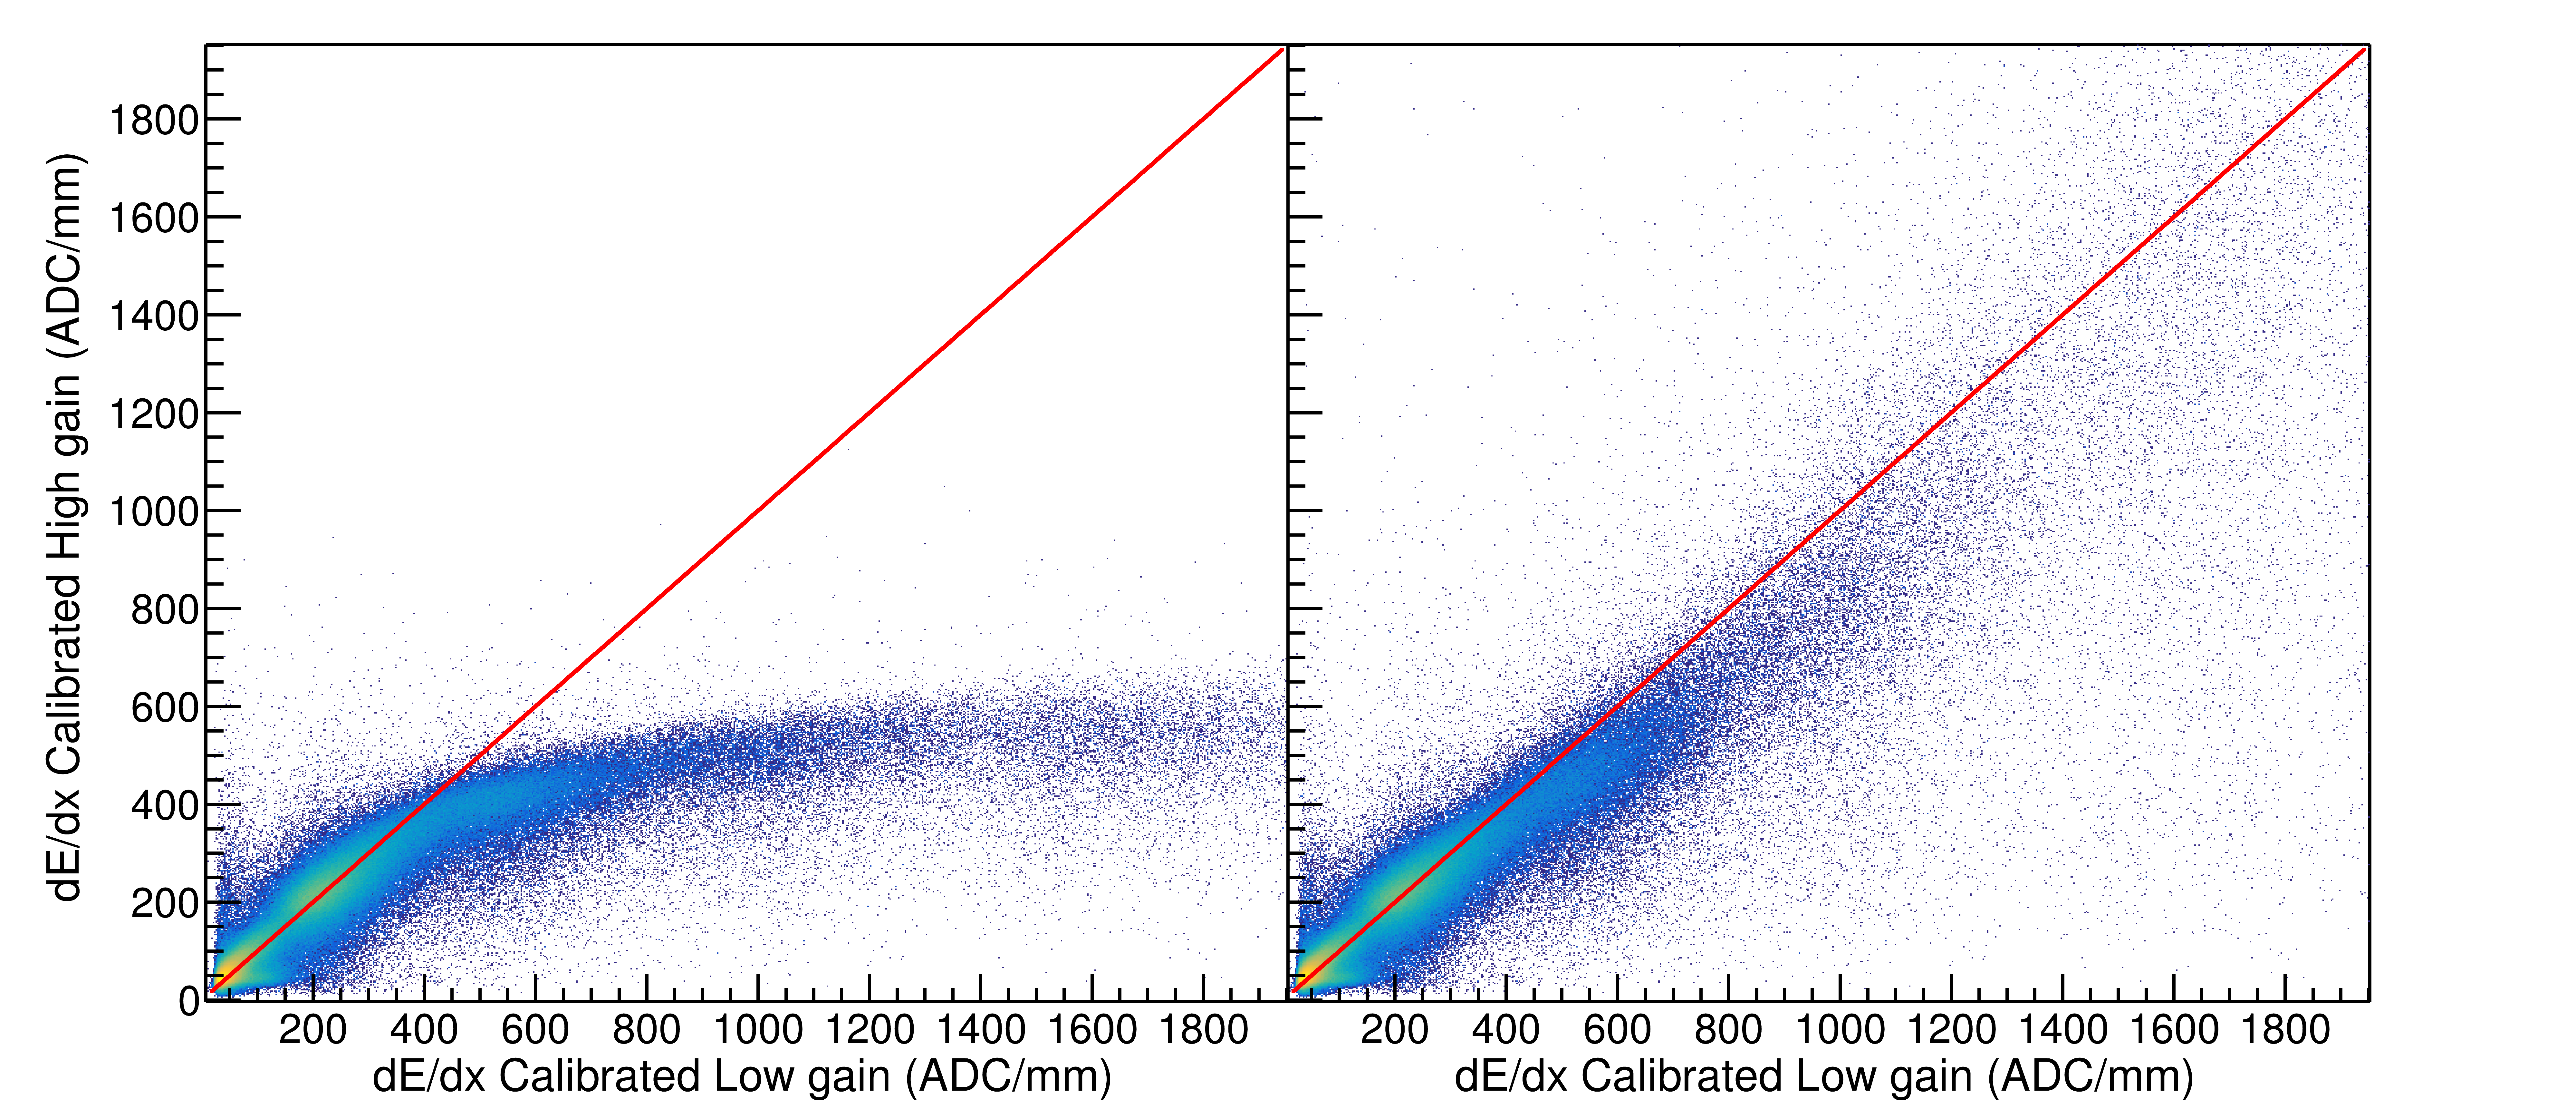
\includegraphics[width=\linewidth]{fig11}
\caption{The left panel shows the high gain stopping power vs low gain when the method of desaturation was not applied. In the right panel the desaturation technique was applied to the high gain region. The low gain does not suffer from saturation and represents the true $dE/dx$ value.}
\label{fig:lowvshigh}
\end{figure*}

\begin{figure*}[t]
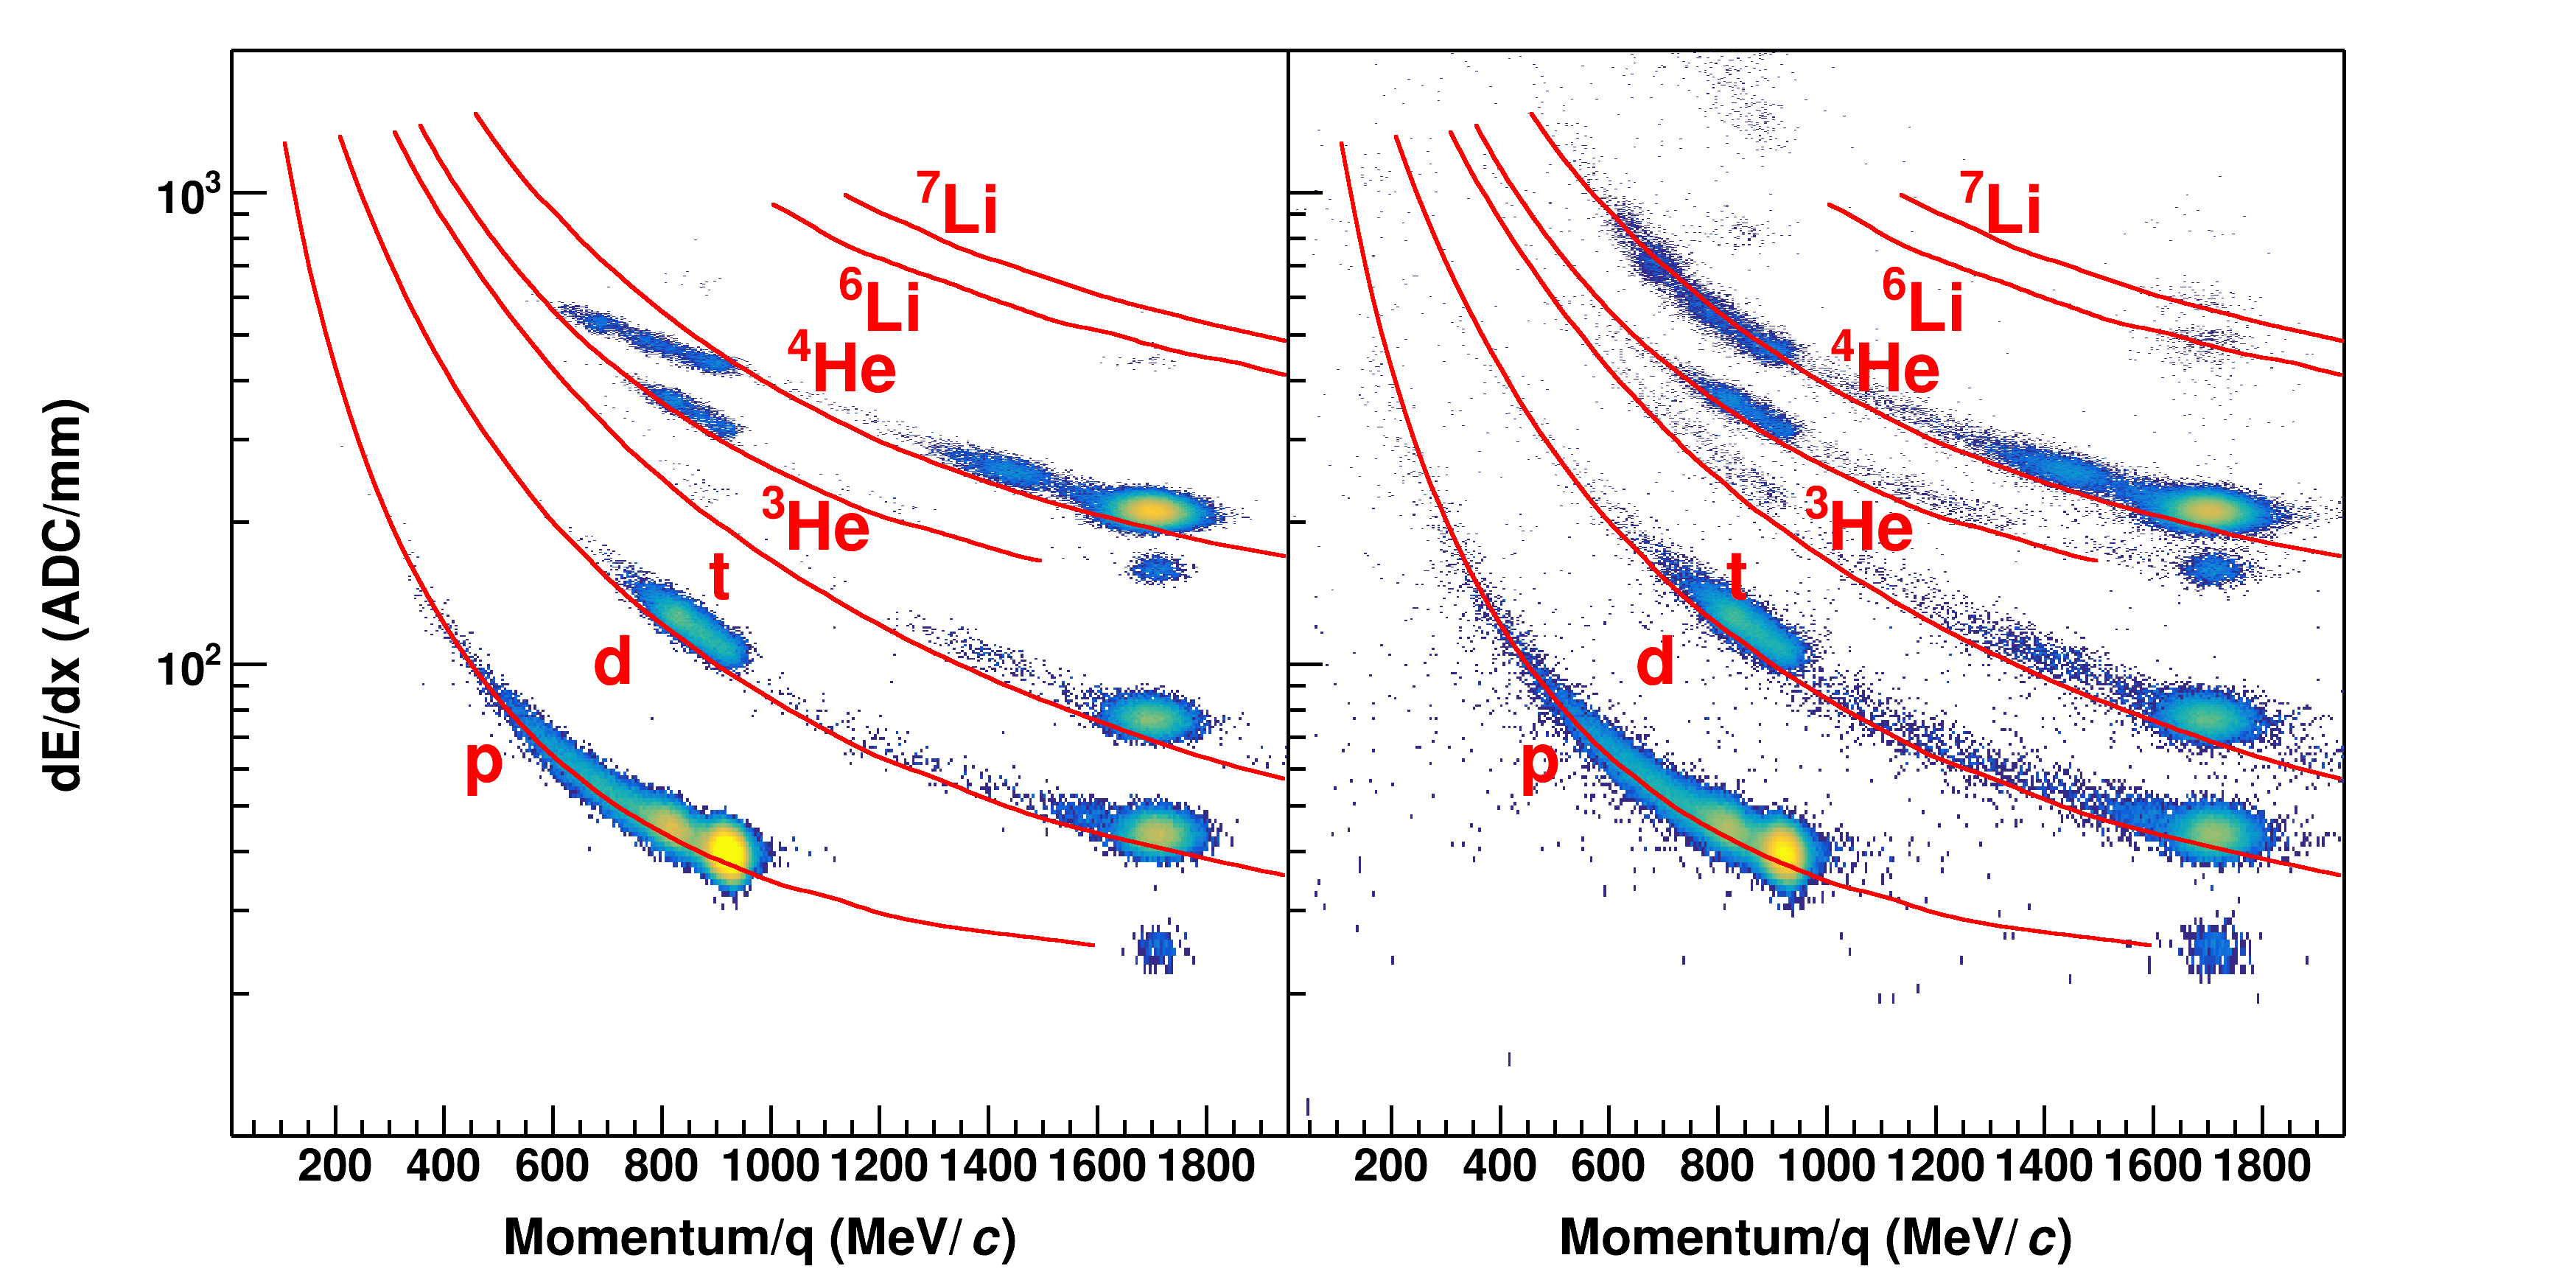
\includegraphics[width=\linewidth]{fig12}
\caption{Uncorrected (left panel) and desaturated (right panel) cocktail data.}
\label{fig:cocktail_combine}
\end{figure*}

\begin{figure*}[t]
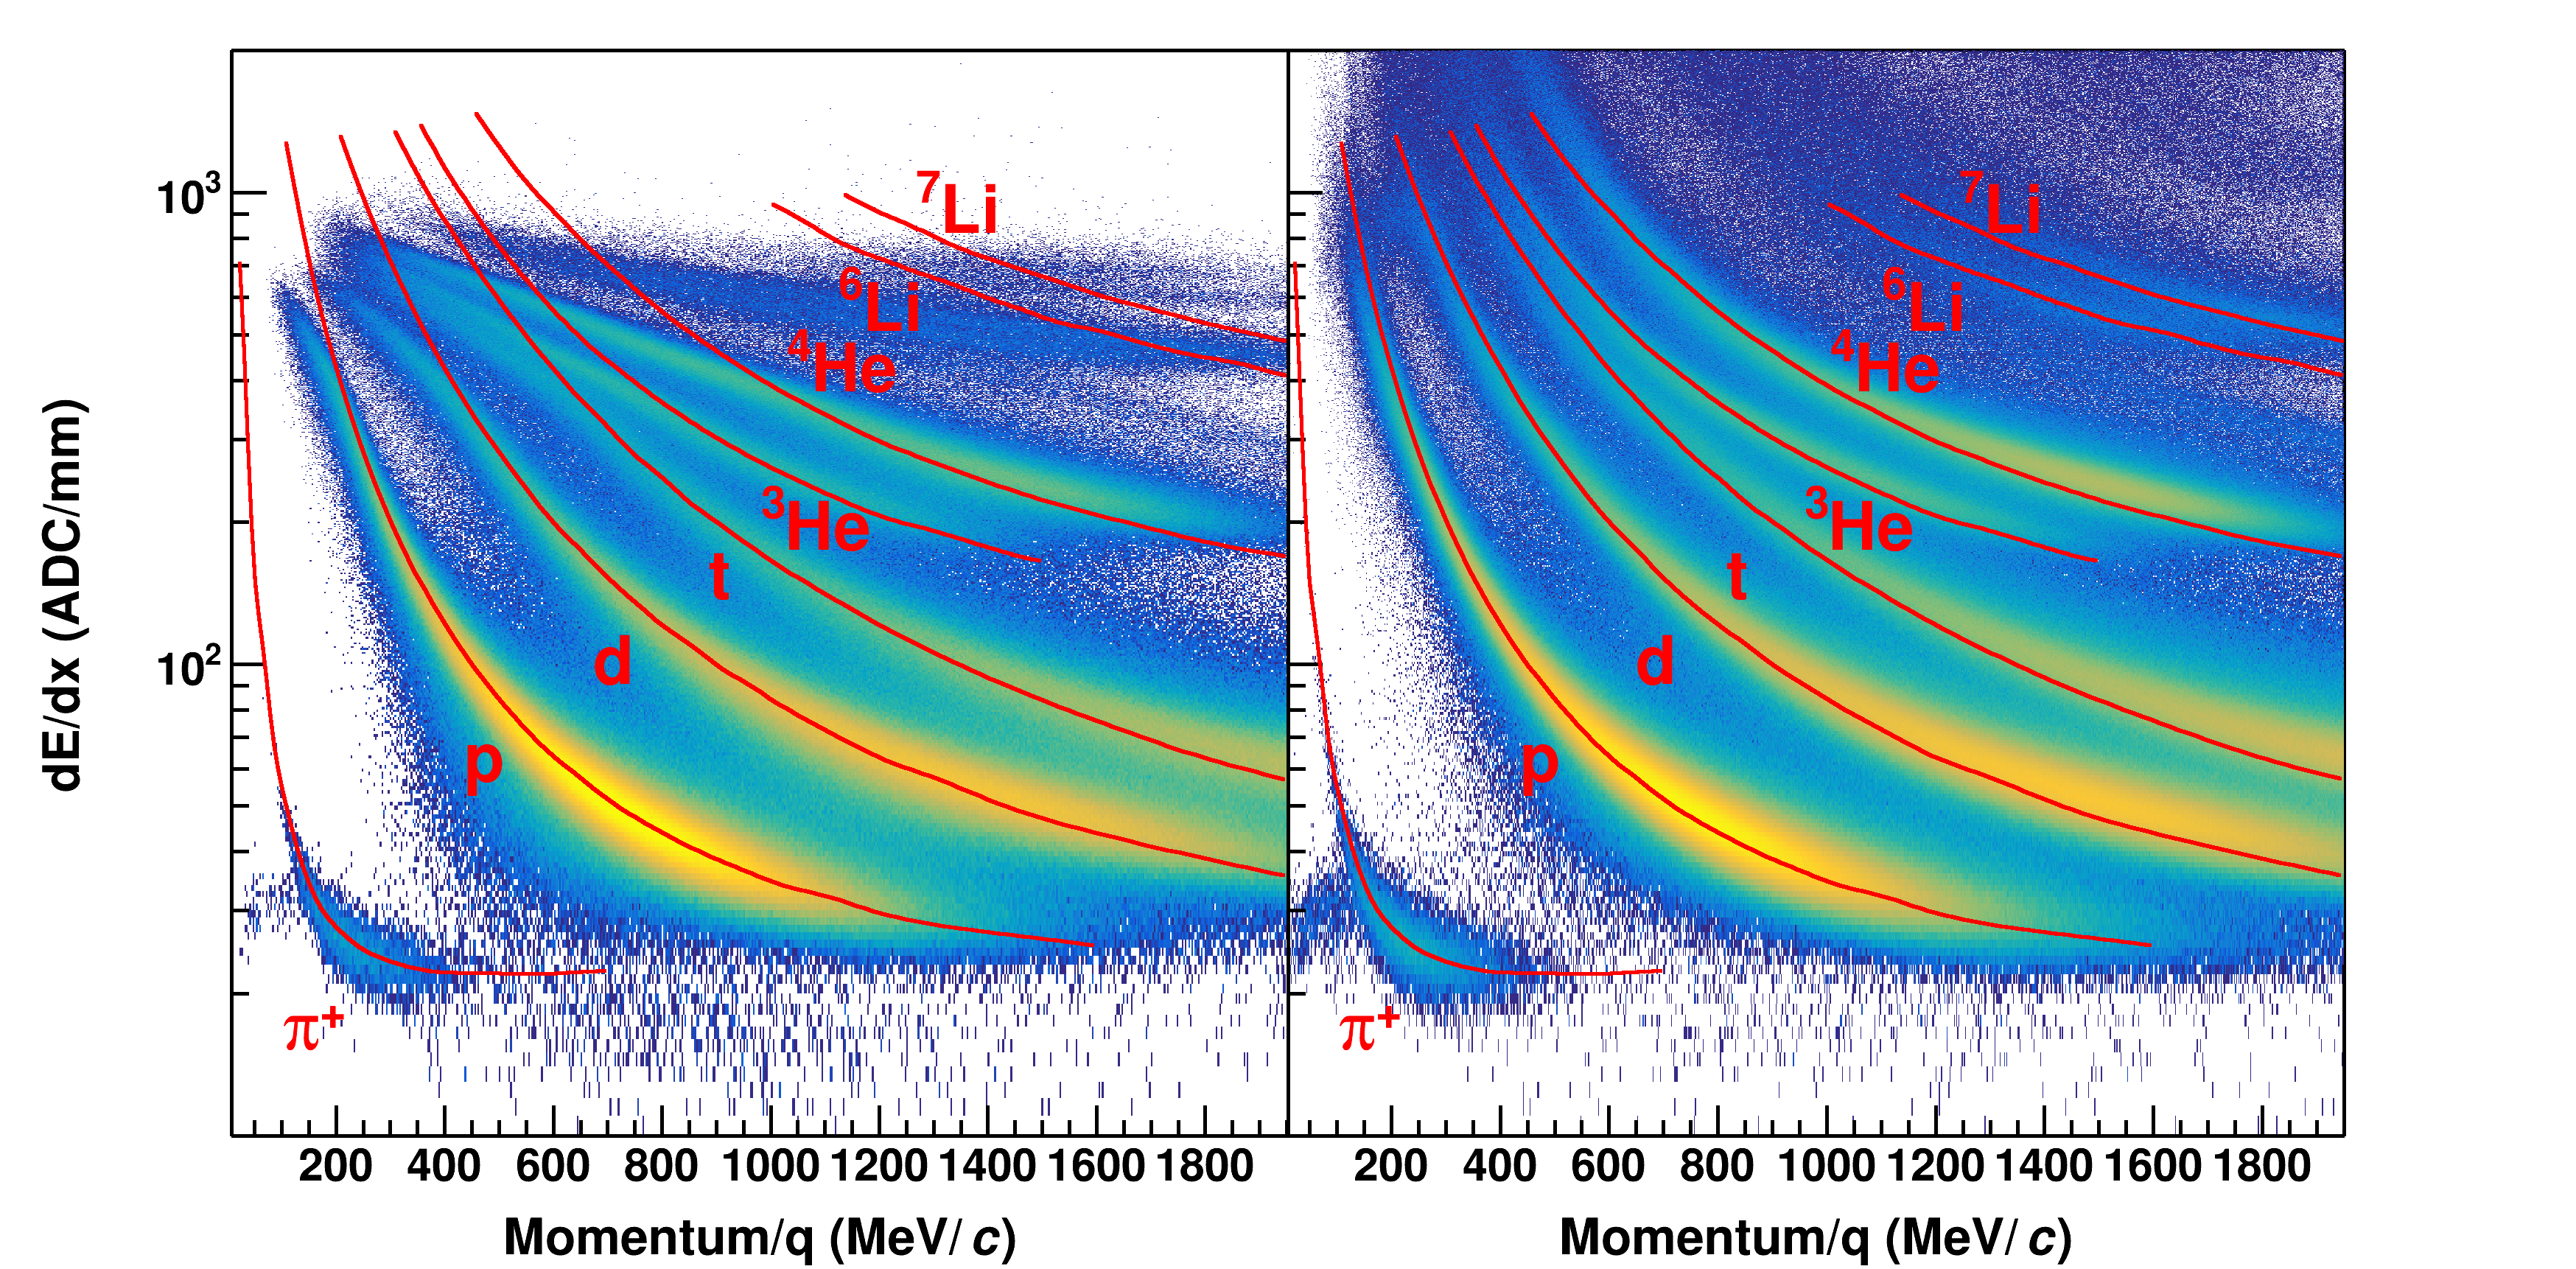
\includegraphics[width=\linewidth]{fig13}
\caption{Uncorrected (left panel) and desaturated (right panel) collision data at polar angles of $\theta < 40^{\circ}$ and azimuthal angles between $-80^{\circ} < \phi < 80^{\circ}$}
\label{fig:data_combine}
\end{figure*}

\section{Results}
\subsection{Low gain vs corrected high gain}

Tracks which saturate pads in the high gain region are not saturated in the low gain region. By comparing the dE/dx values of these two sections, we can directly measure the success of the desaturation in the high gain regions using the method described above.  
 
In Fig.~\ref{fig:lowvshigh}, the effect of saturation can be seen in the high gain region for the uncorrected data. For signals below 400 ADC/mm \footnote{Un-calibrated ADC channels in arbitrary units.} the electronics are not saturated, and therefore the high and low gain sections agree. The data starts to saturate above 400 ADC/mm in the high gain channels eventually reaching a plateau while the low gain sections are not saturated and provide the true $dE/dx$ values.
 After applying the desaturation method, the correlation between the high and low gain sections is restored, as seen in Fig.~\ref{fig:lowvshigh}. From this comparison, we infer that the correction works up to signals of 2000 ADC/mm, increasing the dynamic range by a factor of at least 5.

\subsection{Particle Identification (PID)}


Comparing the low to high gain sections directly validates the desaturation technique, but the goal  of this exercise is to improve the particle identification (PID). In the following PID plots the red lines represent the most probable energy loss as given by Geant4 straggling functions. A linear calibration was performed to convert keV in Geant4 to ADC in the experiment given by $ADC/mm = 19\;keV/cm$.

There are pronounced PID lines of several particle species in both the uncorrected and corrected cocktail beam PID shown in the subplots of Fig.~\ref{fig:cocktail_combine}. Three ovals around a momentum of 1700~MeV/$c$/q and two near 900~MeV/$c$/q correspond to the three $B\rho$ settings injected into the TPC. The tails of the PID lines are resulting from the particles passing through the walls and other materials outside the main detector volume, therefore lowering the initial momentum. 

The uncorrected data in Fig.~\ref{fig:cocktail_combine} shows the effects of saturation; the PID lines deviate from their theoretical expectations starting at around 400~ADC/mm eventually reaching a plateau. After applying the desaturation technique, we see a large improvement, most notably for the He and Li particles, which suffer the most from saturation. A more subtle improvement of the lighter particles, (p, d, t), can also be seen in the PID lines at lower momenta.

Looking at the collision data, shown in Fig.~\ref{fig:data_combine}, we also see a similar result. In the collision data, the PID suffers from more background and inefficiencies than the cocktail beam, nevertheless we can see a similar improvement in the PID lines when comparing before and after applying desaturation. Notably the largest improvement is the separation of particle species at lower momenta and the separation of the Li species into ${}^{6}$Li and ${}^{7}$Li. In these regions, there was little to no PID resolution before desaturation. 

\clearpage

\section{Conclusion}

The saturation  of the electronics reduces $dE/dx$ resolution and even the maximum charge observable inside of a TPC.  We have shown that some of the saturated information is recoverable. Since the Pad Response Function of the TPC is fixed by the anode wire geometries, an experimental PRF can be calculated from the unsaturated experimental data. The charge distribution resulting from an avalanche on a wire must follow this PRF even if the electronics of some channels directly under the avalanche are saturated while the pads farther away are not saturated. By using these unsaturated pads and minimizing a $\chi^2$ fit  to the PRF we recover the unknown saturated charges. This method will not be able to extend the dynamic range in regions of the TPC where the track density is high, such as around the target location, due to the mixing of charges from other tracks. 

The dynamic range was extended by at least a factor of 5, as demonstrated by the improved PID lines, and quantified by direct comparison to low gain sections of the TPC. This improved PID allows us to extend the momentum distributions of all species to lower momenta and to heavier ions than what was previously available. 


\section{Acknowledgments}
This work was supported by the U.S. Department of Energy under Grant Nos.  DE-SC0004835,  DE-SC0014530, DE-NA0002923, DE-FGC2-93ER40773,  US  National Science Foundation Grant  No.  PHY-1565546, the  Japanese  MEXT  KAKENHI (Grant-in-Aid  for  Scientific  Research  on  Innovative  Areas)  grant  No. 24105004, the National Research Foundation of Korea under grant Nos. 2016K1A3A7A09005578, 2018R1A5A1025563,  the Polish National Science Center (NCN), under contract Nos. UMO-2013/09/B/ST2/04064, UMO-2013/-10/M/ST2/00624, and the Robert A. Welch Foundation (A-1266). The computing resources for analyzing the data was provided by the HOKUSAI-GreatWave system at RIKEN and the MSU HPCC and the EMBER cluster at the NSCL. 

\section*{References}

\bibliography{mybibfile}

\end{document}